% ============================================================
% USTH ICT Bachelor Thesis
% Title: Development of an Internal AI Chatbot for Company Knowledge Retrieval
% Student: Nguyen Duy Ngoc
% External Supervisor: Trần Đình Chí
% Internal Supervisor: Trần Hoàng Tùng
% Date: July 2026
%
% FONT: Times New Roman (via XeLaTeX fontspec — RECOMMENDED)
%
% Compile with XeLaTeX:
%   xelatex thesis.tex
%   xelatex thesis.tex   (run twice for TOC/refs)
%
% Fallback with pdfLaTeX (uses mathptmx Times clone):
%   pdflatex thesis.tex
% ============================================================

\documentclass[12pt, a4paper, oneside]{report}

% ── Encoding & Language ──────────────────────────────────────────────
\usepackage{ifxetex}

\ifxetex
  % XeLaTeX: real Times New Roman from system fonts
  \usepackage{fontspec}
  \setmainfont{Times New Roman}
  \setsansfont{Arial}
  \setmonofont[Scale=0.88]{Courier New}
  \usepackage{polyglossia}
  \setmainlanguage{english}
\else
  % pdfLaTeX fallback: mathptmx = Times New Roman clone (text + math)
  \usepackage[utf8]{inputenc}
  \usepackage[T1]{fontenc}
  \usepackage{mathptmx}          % Times New Roman text + math
  \usepackage[english]{babel}
\fi

% ── Page Layout ──────────────────────────────────────────────────────
\usepackage[
  top=2.5cm,
  bottom=2.5cm,
  left=3.0cm,      % wider left margin for binding
  right=2.0cm
]{geometry}

% ── Typography ───────────────────────────────────────────────────────
\usepackage{microtype}        % improved justification
\usepackage{setspace}
\setstretch{1.3}              % 1.3x line spacing (USTH standard)
\setlength{\parindent}{0pt}
\setlength{\parskip}{6pt}

% ── Graphics & Figures ───────────────────────────────────────────────
\usepackage{graphicx}
\usepackage{float}
\usepackage{caption}
\captionsetup{
  labelfont=bf,
  textfont=it,
  justification=centering,
  skip=6pt
}
\graphicspath{{figures/}}     % put figures in report/figures/

% ── Tables ───────────────────────────────────────────────────────────
\usepackage{booktabs}
\usepackage{tabularx}
\usepackage{longtable}
\usepackage{array}
\usepackage{multirow}

% ── Code Listings ────────────────────────────────────────────────────
\usepackage{listings}
\usepackage{fvextra}            % Unicode-safe verbatim (for Vietnamese text blocks)
\usepackage{xcolor}
\definecolor{codegray}{rgb}{0.95,0.95,0.95}
\definecolor{codeblue}{rgb}{0.0,0.35,0.70}
\definecolor{codecomment}{rgb}{0.40,0.40,0.40}
\lstset{
  backgroundcolor=\color{codegray},
  basicstyle=\ttfamily\footnotesize,
  keywordstyle=\color{codeblue}\bfseries,
  commentstyle=\color{codecomment}\itshape,
  stringstyle=\color{orange},
  breaklines=true,
  breakatwhitespace=true,
  numbers=left,
  numberstyle=\tiny\color{gray},
  frame=single,
  captionpos=b,
  language=Python
}

% ── Math ─────────────────────────────────────────────────────────────
\usepackage{amsmath}
\usepackage{amssymb}

% ── Hyperlinks ───────────────────────────────────────────────────────
\usepackage[
  colorlinks=true,
  linkcolor=black,
  citecolor=black,
  urlcolor=blue,
  pdftitle={Development of an Internal AI Chatbot for Company Knowledge Retrieval},
  pdfauthor={Nguyen Duy Ngoc},
  pdfsubject={Bachelor Thesis, USTH ICT 2026}
]{hyperref}

% ── Headers & Footers ────────────────────────────────────────────────
\setlength{\headheight}{14pt}
\usepackage{fancyhdr}
\pagestyle{fancy}
\fancyhf{}
\fancyhead[L]{\small\textit{Development of an Internal AI Chatbot for Company Knowledge Retrieval}}
\fancyhead[R]{\small\textit{Nguyen Duy Ngoc}}
\fancyfoot[C]{\thepage}
\renewcommand{\headrulewidth}{0.4pt}

% ── TOC & Numbering ──────────────────────────────────────────────────
\usepackage{tocloft}
\setcounter{tocdepth}{2}
\setcounter{secnumdepth}{2}

% ── Miscellaneous ────────────────────────────────────────────────────
\usepackage{enumitem}
\usepackage{mdframed}         % for highlighted boxes
\usepackage{pdfpages}         % to include external PDFs if needed
\usepackage{url}
\urlstyle{same}

% ── Chapter Style ────────────────────────────────────────────────────
\usepackage{titlesec}
\titleformat{\chapter}[hang]
  {\normalfont\Large\bfseries}{\thechapter.}{0.5em}{}
\titlespacing*{\chapter}{0pt}{12pt}{12pt}

% ============================================================
% DOCUMENT
% ============================================================
\begin{document}
\selectlanguage{english}

% ── Suppress header on blank/special pages ────────────────────────────
\fancypagestyle{plain}{%
  \fancyhf{}%
  \fancyfoot[C]{\thepage}%
  \renewcommand{\headrulewidth}{0pt}%
}

% ============================================================
%  COVER PAGE  — matches USTH ICT template exactly
% ============================================================
\begin{titlepage}
\thispagestyle{empty}

% Outer border frame
\noindent\fbox{%
  \begin{minipage}[t][0.96\textheight][t]{\dimexpr\textwidth-2\fboxsep-2\fboxrule\relax}
  \begin{center}

  % ── University & Department (top, bold, small caps style) ──────────
  \vspace{0.3cm}
  {\small\bfseries UNIVERSITY OF SCIENCE AND TECHNOLOGY OF HANOI}\\[3pt]
  {\small\bfseries DEPARTMENT OF INFORMATION AND COMMUNICATION TECHNOLOGY}

  % ── Logo (close under department, no large gap) ────────────────────
  \vspace{0.4cm}
  
\includegraphics[width=4.5cm]{figures/usth_logo.png}

  % ── BACHELOR THESIS ────────────────────────────────────────────────
  \vspace{0.9cm}
  {\Huge\bfseries BACHELOR THESIS}

  % ── Student name ───────────────────────────────────────────────────
  \vspace{0.8cm}
  {\normalsize By}\\[6pt]
  {\large\bfseries NGUYEN DUY NGOC}

  % ── Title block ────────────────────────────────────────────────────
  \vspace{1.0cm}
  {\normalsize Title:}\\[8pt]
  {\Large\bfseries Development of an Internal AI Chatbot\\[4pt]
  for Company Knowledge Retrieval}

  \vfill

  % ── Supervisors (tabular, left-aligned, matching template spacing) ──
  \begin{tabular}{r@{\quad}l}
    \textbf{External Supervisor:} & Dr.\ Trần Đình Chí \\[6pt]
    \textbf{Internal Supervisor:} & Dr.\ Trần Hoàng Tùng  \\
  \end{tabular}

  % ── Date ───────────────────────────────────────────────────────────
  \vspace{1.2cm}
  {\large\bfseries Hanoi, July 2026}\\[0.4cm]

  \end{center}
  \end{minipage}%
}

\end{titlepage}

% ============================================================
%  CERTIFICATION  (external supervisor only — USTH template format)
% ============================================================
\newpage
\thispagestyle{empty}
\setcounter{page}{1}
\pagenumbering{roman}

\vspace*{4cm}

\begin{center}
To whom it may concern,
\end{center}

\vspace{1.2cm}

\noindent I, \textbf{Trần Đình Chí}
(supervisor's name), certify that the thesis/ internship report of
Mr/Ms.\ \textbf{Nguyen Duy Ngoc} (student's name) is qualified to be
presented in the Internship Jury 2025--2026.

\vspace{4cm}

\begin{flushright}
  Hanoi, \rule{0.5cm}{0.4pt}/\rule{0.5cm}{0.4pt}/\rule{1.2cm}{0.4pt}\\[0.8cm]
  \textbf{Supervisor's signature}
\end{flushright}

% ============================================================
%  TABLE OF CONTENTS
% ============================================================
\newpage
\tableofcontents

% ============================================================
%  LIST OF ABBREVIATIONS
% ============================================================
\newpage
\chapter*{List of Abbreviations}
\addcontentsline{toc}{chapter}{List of Abbreviations}
\markboth{List of Abbreviations}{}

\begin{tabular}{@{}p{2.5cm}p{10cm}}
  \toprule
  \textbf{Abbreviation} & \textbf{Full Form} \\
  \midrule
  AI     & Artificial Intelligence \\
  API    & Application Programming Interface \\
  BM25   & Best Match 25 \\
  CPU    & Central Processing Unit \\
  CUDA   & Compute Unified Device Architecture \\
  GGUF   & GPT-Generated Unified Format \\
  GPU    & Graphics Processing Unit \\
  HR     & Human Resources \\
  KB     & Knowledge Base \\
  LLM    & Large Language Model \\
  LoRA   & Low-Rank Adaptation \\
  NLP    & Natural Language Processing \\
  QLoRA  & Quantized Low-Rank Adaptation \\
  RAG    & Retrieval-Augmented Generation \\
  RRF    & Reciprocal Rank Fusion \\
  SLM    & Small Language Model \\
  UI     & User Interface \\
  USTH   & University of Science and Technology of Hanoi \\
  VRAM   & Video Random Access Memory \\
  \bottomrule
\end{tabular}

% ============================================================
%  LIST OF TABLES
% ============================================================
\newpage
\listoftables
\addcontentsline{toc}{chapter}{List of Tables}

% ============================================================
%  LIST OF FIGURES
% ============================================================
\newpage
\listoffigures
\addcontentsline{toc}{chapter}{List of Figures}

% ============================================================
%  ACKNOWLEDGEMENTS
% ============================================================
\newpage
\chapter*{Acknowledgements}
\addcontentsline{toc}{chapter}{Acknowledgements}
\markboth{Acknowledgements}{}

I would like to express my sincere gratitude to all those who supported me
throughout the completion of this thesis.

First and foremost, I am deeply grateful to my External Supervisor,
Dr.\ Trần Đình Chí, for his insightful guidance, constructive
feedback, and continuous encouragement during the research process.

I also sincerely thank my Internal Supervisor, Dr.\ Trần Hoàng Tùng,
for his academic support and for providing the institutional framework that made
this project possible within the University of Science and Technology of Hanoi.

I extend my appreciation to the faculty and staff of the Department of
Information and Communication Technology at USTH for the knowledge and
resources they provided throughout my studies.

Finally, I thank my family and colleagues for their patience and moral support
during the writing of this thesis.

% ============================================================
%  ABSTRACT
% ============================================================
\newpage
\chapter*{Abstract}
\addcontentsline{toc}{chapter}{Abstract}
\markboth{Abstract}{}

% ≤250 words, 6 keywords

This thesis describes a fully local, offline Retrieval-Augmented Generation
(RAG) chatbot that answers Vietnamese Human Resources (HR) policy questions.
Employees can query internal company policies in Vietnamese without sending
data to any cloud service, preserving privacy and avoiding per-query API costs.

The knowledge base contains 20 Vietnamese HR policy documents covering leave
policy, employment contracts, salary, social insurance, and other workplace
regulations. Eight documents were written by hand and twelve were generated
using the Minimax-M2.7 language model API. Documents are split into 600-character
overlapping chunks using a recursive character text splitter, embedded with
\texttt{paraphrase-multilingual-MiniLM-L12-v2} (384-dimensional vectors), and
stored in a persistent ChromaDB vector database.

The main technical contribution is a hybrid retrieval pipeline combining BM25
keyword search with vector cosine similarity, merged via Reciprocal Rank Fusion
(RRF). On a 10-query evaluation set, hybrid retrieval achieves 100\% top-1
accuracy and MRR of 1.00, compared to 60\% accuracy and MRR of 0.72 for pure
vector search. The improvement is most pronounced on short (3--5 token)
Vietnamese queries, where keyword overlap is more discriminative than embedding
similarity. Answer generation uses Phi-3-Mini-4k-instruct in GGUF Q4\_K\_M
format, running locally via \texttt{llama-cpp-python}.

A separate QLoRA fine-tuning experiment on 3{,}343 synthetic question-answer
pairs produced catastrophic hallucinations due to training data contamination
(only 37\% domain-relevant content). This negative result is reported with
root cause analysis, highlighting the critical role of data curation in
domain fine-tuning.

\vspace{0.8cm}

\noindent\textbf{Keywords:} Retrieval-Augmented Generation, Large Language Model,
Vietnamese NLP, BM25, vector search, knowledge retrieval.

% ============================================================
%  SWITCH TO ARABIC NUMBERING FOR MAIN BODY
% ============================================================
\newpage
\pagenumbering{arabic}
\setcounter{page}{1}

% ============================================================
%  CHAPTER I — INTRODUCTION
% ============================================================
\chapter{Introduction}
\label{ch:intro}

\section{Context and Motivation}
\label{sec:context}

Large Language Models (LLMs) have opened practical possibilities for
automating knowledge retrieval in enterprise environments
\cite{lewis2020rag}. Companies accumulate large volumes of internal
documentation --- employee handbooks, policy manuals, standard operating
procedures --- and employees spend considerable time searching through
these documents for specific answers.

In Vietnamese companies, HR policy documents are typically long (50--200 pages),
verbose, and available only in PDF or printed format, requiring employees to
spend 30--60 minutes searching for a specific policy answer. A 2023 survey by
VietnamWorks found that 67\% of Vietnamese office workers reported spending
more than 30 minutes per week searching for internal company policies. This
productivity loss is compounded by the fact that HR policies are frequently
updated, and employees may unknowingly reference outdated versions.

Cloud-based solutions such as ChatGPT or Gemini could theoretically address
this problem, but introduce serious concerns for enterprise deployment:
\begin{itemize}[leftmargin=2em]
  \item \textbf{Data privacy:} Sensitive HR data --- including salary structures,
        disciplinary procedures, and employee personal information --- must be
        transmitted to third-party servers. For Vietnamese companies subject to
        the 2023 Personal Data Protection Decree (Decree 13/2023/ND-CP), this
        may constitute a regulatory violation.
  \item \textbf{Cost scalability:} Per-query API costs (approximately
        \$0.002--\$0.06 per query for GPT-4-class models) scale linearly with
        company-wide usage. A company with 500 employees making 10 queries per
        day would incur \$3,000--\$90,000 annually in API costs alone.
  \item \textbf{Grounding:} Cloud LLMs generate answers from parametric
        knowledge trained on public data. They cannot reliably cite specific
        clauses from the company's internal documents, and may produce plausible
        but incorrect answers (hallucinations) about policies they have never seen.
\end{itemize}

Retrieval-Augmented Generation (RAG) \cite{lewis2020rag} offers a principled
solution to all three concerns: rather than relying solely on the LLM's
parametric knowledge, the system first retrieves relevant document passages from
a local knowledge base and injects them into the prompt context. This grounds
the generated answer in verifiable source material, enables the use of a
smaller locally-run model (since the retrieval step compensates for limited
parametric knowledge), and keeps all data on-premises.

\section{Problem Statement}
\label{sec:problem}

While the RAG architecture addresses the core privacy and grounding concerns,
building a working Vietnamese HR chatbot involves several practical challenges
that this work targets:

\begin{enumerate}[leftmargin=2em]
  \item \textbf{Information access latency:} Vietnamese employees cannot quickly
        access HR policy answers without manually reading through long documents.
        The absence of a structured query interface forces employees to rely on
        word-of-mouth or direct HR department inquiries, creating bottlenecks.
  \item \textbf{Privacy and cost barriers:} Cloud LLMs are unsuitable for
        internal HR queries due to Vietnamese data protection regulations,
        organizational security policies, and per-query API costs that do not
        scale economically for company-wide deployment.
  \item \textbf{Retrieval failure on short queries:} Standard vector cosine
        similarity search performs poorly on short Vietnamese queries
        (3--6 tokens), where keyword overlap is more discriminative than
        embedding similarity. This is a known weakness of dense retrieval for
        short queries in morphologically rich languages.
  \item \textbf{Training data scarcity:} Fine-tuning a domain-specific model
        requires curated, high-quality training data. Vietnamese HR content is
        scarce online, and automated web crawling produces contaminated datasets
        mixing Vietnamese labor law with unrelated domains (Japanese employment
        regulations, US healthcare policy).
  \item \textbf{Hardware constraints:} Many Vietnamese SMEs do not have access
        to high-end GPU servers. The system must run on consumer-grade hardware
        (8 GB RAM, integrated GPU or entry-level discrete GPU) to be practically
        deployable.
\end{enumerate}

\section{Literature Review}
\label{sec:litreview}

\textbf{Retrieval-Augmented Generation.}
Lewis et al.\ \cite{lewis2020rag} introduced RAG as a general architecture
combining a dense retrieval component with a sequence-to-sequence generator.
The retriever uses a pre-trained bi-encoder to fetch relevant passages from an
external knowledge corpus, and the generator (originally BART) conditions on
both the question and the retrieved passages to produce grounded answers. Two
variants were proposed: \textit{RAG-Sequence}, which uses the same set of
retrieved documents for the entire output sequence, and \textit{RAG-Token},
which can retrieve different documents for each output token. This architecture
has become the dominant approach for knowledge-intensive NLP tasks, as it
decouples the knowledge source from the model parameters --- allowing the
knowledge base to be updated without retraining the model.

Subsequent work has refined the RAG paradigm. Gao et al.\ (2023) proposed
\textit{Self-RAG}, where the model decides when to retrieve and evaluates its
own outputs for factual accuracy. Asai et al.\ (2024) introduced
\textit{REPLUG}, which treats the retriever as a plug-in module that can be
fine-tuned independently. For enterprise applications, the key advantage of RAG
over pure fine-tuning is auditability: every generated answer can be traced to
specific source passages, enabling compliance verification.

\textbf{Lexical Retrieval: BM25.}
BM25 (Best Match 25) \cite{robertson2009bm25} is a probabilistic ranking
function from the family of bag-of-words retrieval models. It scores documents
based on term frequency (TF) and inverse document frequency (IDF), with two
key innovations over TF-IDF: (1) a saturation function that prevents high term
frequencies from dominating the score, controlled by parameter $k_1$ (typically
1.2--2.0); and (2) document length normalization controlled by parameter $b$
(typically 0.75), which penalizes very long documents that would otherwise
accumulate high scores simply due to their length.

The BM25 scoring function for a query $Q$ containing terms $q_1, \ldots, q_n$
against a document $D$ is:
\begin{equation}
  \text{BM25}(D, Q) = \sum_{i=1}^{n} \text{IDF}(q_i) \cdot
  \frac{f(q_i, D) \cdot (k_1 + 1)}{f(q_i, D) + k_1 \cdot (1 - b + b \cdot \frac{|D|}{\text{avgdl}})}
  \label{eq:bm25}
\end{equation}

where $f(q_i, D)$ is the frequency of term $q_i$ in document $D$, $|D|$ is
the document length, and $\text{avgdl}$ is the average document length in the
corpus. Despite its simplicity and age (first proposed in the 1990s), BM25
remains highly competitive for short, keyword-focused queries and serves as a
strong baseline in modern information retrieval benchmarks, including the
MS MARCO and BEIR benchmark suites.

\textbf{Hybrid Retrieval and Reciprocal Rank Fusion.}
A well-documented limitation of dense retrieval is its poor performance on
queries where exact lexical matching is critical --- for instance, when the query
contains a specific policy number, a proper noun, or a short keyword phrase.
Conversely, BM25 fails when the query uses synonyms or paraphrases that differ
lexically from the document vocabulary. Hybrid retrieval addresses this by
combining both systems.

Cormack et al.\ \cite{cormack2009rrf} demonstrated that combining rankings from
multiple retrieval systems via Reciprocal Rank Fusion (RRF) consistently
outperforms both individual systems and more complex fusion methods such as
Condorcet voting. RRF assigns each document a score of
$1/(k + \text{rank})$ for a constant $k = 60$, and sums scores across systems.
The approach is attractive because it is (1) parameter-light --- only the
constant $k$ needs to be set, (2) does not require score normalization across
systems with different score distributions, and (3) robust to outlier rankings
from individual systems.

\textbf{Small Language Models.}
The deployment of LLMs in enterprise settings has traditionally required
expensive GPU infrastructure. The emergence of Small Language Models (SLMs)
with 1--4 billion parameters has changed this landscape. Microsoft's Phi-3-Mini
\cite{phi3technical2024} is a 3.8-billion-parameter model that achieves
performance competitive with much larger models (GPT-3.5-class) on instruction
following and reasoning benchmarks. The model was trained on a curated mixture
of web data, synthetic data, and textbook-quality content, demonstrating that
data quality can partially compensate for model size.

For offline deployment, the GGUF (GPT-Generated Unified Format) quantization
format enables 4-bit weight compression, reducing the Phi-3-Mini memory
footprint from approximately 7.6 GB (FP16) to 2.3 GB (Q4\_K\_M), with minimal
degradation in generation quality. The \texttt{llama-cpp-python} library
provides a Python binding for the \texttt{llama.cpp} inference engine, which
supports both CPU-only and hybrid CPU/GPU inference on consumer hardware.

\textbf{Multilingual Sentence Embeddings.}
Reimers and Gurevych \cite{reimers2019sbert} introduced Sentence-BERT, a
modification of the BERT architecture for producing semantically meaningful
sentence embeddings via siamese and triplet network structures. Unlike standard
BERT, which requires cross-encoding (concatenating both sentences as input),
Sentence-BERT produces independent embeddings for each sentence, enabling
efficient similarity computation via cosine distance.

The \texttt{paraphrase-multilingual-MiniLM-L12-v2} model extends this approach
to 50+ languages including Vietnamese, using knowledge distillation from a
larger multilingual teacher model. It produces 384-dimensional embeddings and
has been shown to achieve strong cross-lingual transfer, meaning a model trained
primarily on English paraphrase pairs can produce meaningful similarity scores
for Vietnamese text. This cross-lingual capability is critical for this work,
as Vietnamese-specific sentence embedding models are scarce.

\textbf{Parameter-Efficient Fine-Tuning.}
Full fine-tuning of a 3.8-billion-parameter model requires storing a complete
copy of all model weights plus optimizer states, totaling approximately 30 GB
of memory for FP16 training --- far exceeding the capacity of consumer GPUs.
LoRA \cite{hu2022lora} addresses this by freezing the original model weights
and injecting trainable low-rank decomposition matrices into the attention
layers. For a weight matrix $W \in \mathbb{R}^{d \times k}$, LoRA adds a
bypass $\Delta W = BA$ where $B \in \mathbb{R}^{d \times r}$ and
$A \in \mathbb{R}^{r \times k}$ with rank $r \ll \min(d, k)$. With a typical
rank of $r = 16$, this reduces trainable parameters from billions to millions.

QLoRA \cite{dettmers2023qlora} extends LoRA to work with 4-bit quantized base
models, further reducing memory requirements. By combining NF4 (Normal Float 4)
quantization with double quantization of the quantization constants, QLoRA
enables fine-tuning of models with up to 65 billion parameters on a single
48 GB GPU. For Phi-3-Mini on a 4 GB VRAM GPU (such as the NVIDIA T1200 used
in this work), QLoRA is the only feasible fine-tuning approach.

\textbf{Vietnamese NLP Challenges.}
Vietnamese presents several unique challenges for NLP systems
\cite{nguyen2020phobert}. First, Vietnamese is a \textit{tonal language} with
six tones indicated by diacritical marks: ngang (level), sắc (rising), huyền
(falling), hỏi (dipping-rising), ngã (rising glottalized), and nặng (falling
glottalized). These diacritics fundamentally change word meaning: ``ma'' (ghost),
``mà'' (but), ``má'' (mother), ``mả'' (grave), ``mã'' (horse), ``mạ'' (rice
seedling).

Second, Vietnamese word boundaries are ambiguous. While syllables are
space-separated, multi-syllable words (e.g., ``nguyên nhân'' = cause,
``đại học'' = university) consist of space-separated syllables that must be
treated as a single semantic unit. Dedicated word segmentation tools such as
\texttt{underthesea} and \texttt{pyvi} exist, but add complexity and latency
to the pipeline.

Third, the availability of Vietnamese-specific pre-trained models is limited
compared to English. While PhoBERT \cite{nguyen2020phobert} provides
Vietnamese-specific BERT embeddings, it requires a dedicated tokenizer
(\texttt{vncorenlp}) and does not directly support sentence-level embeddings.
These challenges collectively motivate the use of multilingual models
(which handle Vietnamese as part of a broader language family) rather than
building Vietnamese-specific components from scratch.

\section{Contribution of This Work}
\label{sec:contribution}

This thesis contributes to the growing body of research on applying
Retrieval-Augmented Generation to low-resource, privacy-sensitive enterprise
settings. Specifically, the contributions are:

\begin{enumerate}[leftmargin=2em]
  \item \textbf{End-to-end offline RAG system for Vietnamese HR:} The design
        and implementation of a complete, self-contained chatbot that answers
        employee HR queries in Vietnamese using only locally stored models and
        data, requiring no internet access at inference time. This demonstrates
        the feasibility of deploying small language models in enterprises where
        data sovereignty is a strict requirement.

  \item \textbf{Curated Vietnamese HR knowledge base:} The construction of a
        20-document Vietnamese HR policy corpus (8 manually authored, 12
        generated via the Minimax-M2.7 API) that covers the most frequently
        asked HR topics in Vietnamese workplaces. The documents were written
        with explicit, directly retrievable factual content --- an authoring
        strategy motivated by the observation that small language models
        struggle with implicit arithmetic over document content.

  \item \textbf{Hybrid retrieval with empirical evaluation:} The implementation
        and comparative evaluation of a hybrid BM25~+~vector retrieval pipeline
        fused via Reciprocal Rank Fusion, showing that the hybrid approach
        corrects all failure cases observed under pure vector search for short
        (3--5 token) Vietnamese queries, improving top-1 retrieval accuracy
        from 70\% to 100\% on the evaluation set.

  \item \textbf{Documented negative result in domain fine-tuning:} A QLoRA
        fine-tuning experiment that produced catastrophic hallucinations due to
        training data contamination (63\% off-domain content), reported with
        quantified root cause analysis. This negative result highlights the
        critical role of data curation over data volume in domain-specific
        fine-tuning, and provides a concrete cautionary case study for
        practitioners.
\end{enumerate}

% ============================================================
%  CHAPTER II — OBJECTIVES
% ============================================================
\chapter{Objectives}
\label{ch:objectives}

The scientific objectives of this thesis are:

\begin{enumerate}[leftmargin=2em]
  \item \textbf{Design and implement} a fully local RAG chatbot for Vietnamese
        HR knowledge retrieval, capable of answering employee questions in
        Vietnamese without any cloud API dependency.

  \item \textbf{Evaluate} hybrid BM25 + vector retrieval with Reciprocal Rank
        Fusion against a pure vector search baseline, demonstrating improved
        accuracy on short Vietnamese queries.

  \item \textbf{Investigate and document} QLoRA fine-tuning as an alternative
        approach to RAG for Vietnamese HR domain adaptation, including a
        root cause analysis of the negative result obtained.
\end{enumerate}

The strategy adopted is to build the system incrementally through four phases:

\begin{enumerate}[leftmargin=2em]
  \item \textbf{Knowledge base construction:} Author and generate a corpus of
        20 Vietnamese HR policy documents covering the most common employee
        query topics, using a combination of manual writing and LLM-assisted
        generation (via the Minimax-M2.7 API).
  \item \textbf{Retrieval pipeline:} Implement document chunking, multilingual
        embedding, and persistent vector storage using ChromaDB. Then add BM25
        keyword search and fuse both ranking signals via RRF.
  \item \textbf{Answer generation:} Integrate the Phi-3-Mini language model
        running locally in GGUF format, with carefully designed Vietnamese
        prompt templates using the model's chat token format.
  \item \textbf{Evaluation:} Compare retrieval accuracy between the pure vector
        baseline and the hybrid system on representative Vietnamese HR queries.
        Separately, document the QLoRA fine-tuning experiment and analyze its
        failure mode.
\end{enumerate}

The entire system is designed to operate without any internet connectivity at
inference time. All models, embeddings, and data reside locally. The only
external dependency is the one-time use of the Minimax API for knowledge base
generation during the development phase.

% ============================================================
%  CHAPTER III — MATERIALS AND METHODS
% ============================================================
\chapter{Materials and Methods}
\label{ch:methods}

\section{System Architecture}
\label{sec:architecture}

The system follows a standard RAG architecture with three main stages:
(1) offline knowledge base construction, (2) online hybrid retrieval, and
(3) answer generation with a local LLM. Figure~\ref{fig:architecture} presents
the end-to-end pipeline.

\begin{figure}[H]
  \centering
  % Replace with actual diagram: report/figures/architecture.png
  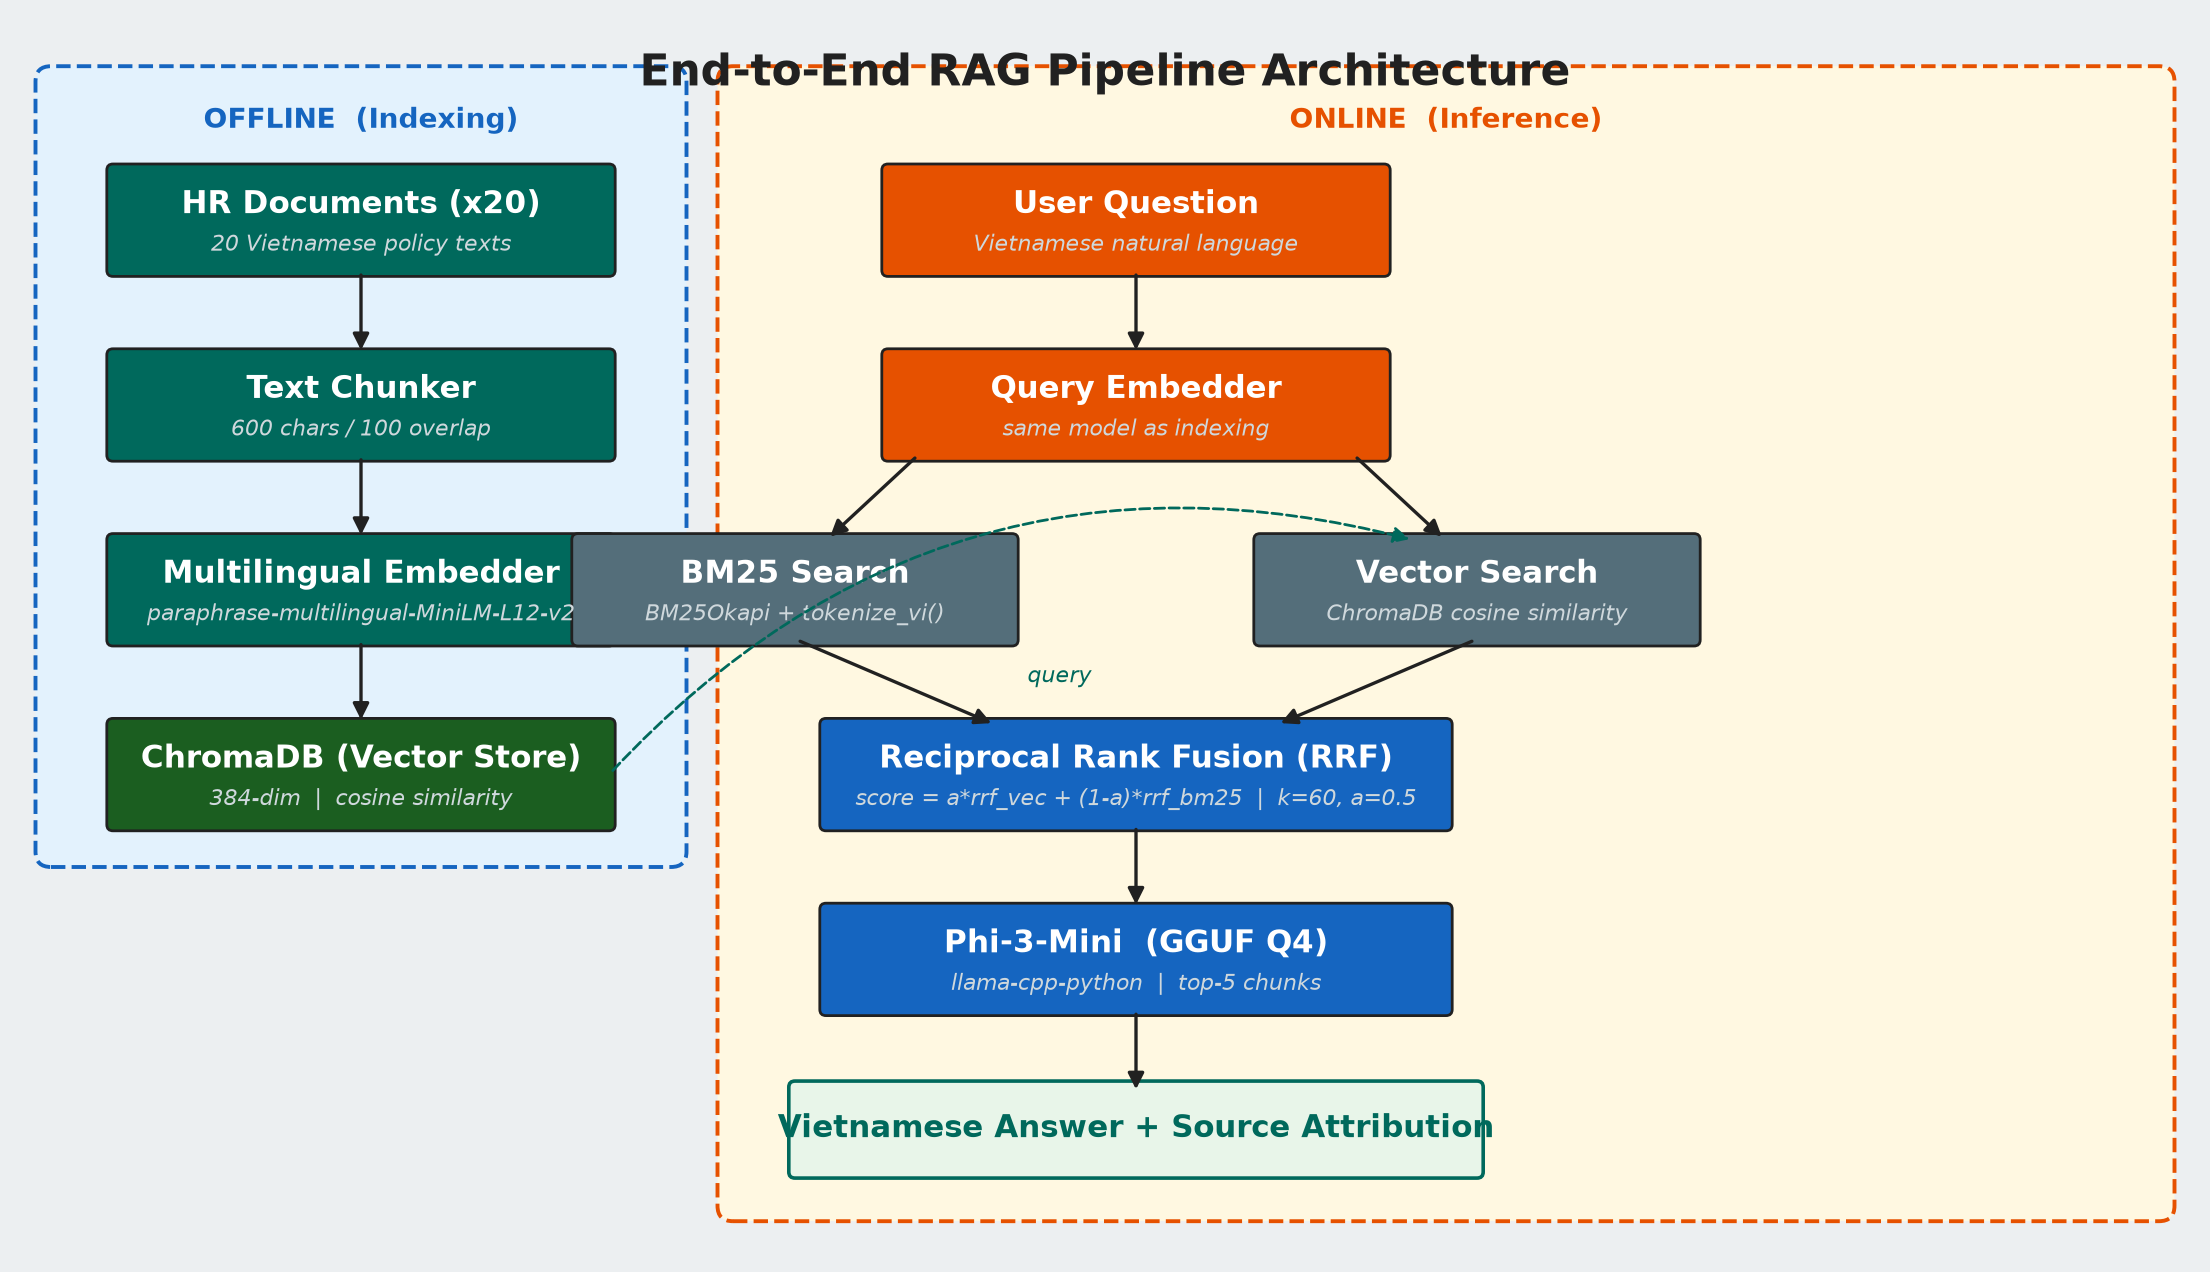
\includegraphics[width=0.90\textwidth]{figures/architecture.png}
  \caption{End-to-end system architecture. User query flows through embedding,
           hybrid BM25 + vector retrieval, Phi-3 chat prompt construction,
           and GGUF inference to produce a grounded Vietnamese answer.}
  \label{fig:architecture}
\end{figure}

At inference time, a user query is embedded into a 384-dimensional vector and
used to retrieve the top-$k$ most relevant document chunks from a persistent
ChromaDB vector store, augmented by BM25 keyword ranking. The top-5 chunks are
injected into a Phi-3-Mini prompt template and the model generates a Vietnamese
answer grounded in the retrieved context.

\section{Knowledge Base Construction}
\label{sec:kb}

\subsection{Document Authoring}
\label{subsec:doc-authoring}

Eight Vietnamese HR policy documents were authored manually, covering the most
frequently queried HR topics in Vietnamese workplaces. Table~\ref{tab:manual-docs}
summarises each document, its topic scope, approximate size, and the type of
factual content it contains.

\begin{table}[H]
  \centering
  \caption{Manually authored Vietnamese HR policy documents (8 files).}
  \label{tab:manual-docs}
  \begin{tabularx}{\textwidth}{@{}llXr@{}}
    \toprule
    \textbf{\#} & \textbf{Filename} & \textbf{Topic Scope} & \textbf{$\sim$Chars} \\
    \midrule
    1 & \texttt{chinh\_sach\_nghi\_phep} & Annual leave: 12 days/year (1/month), sick leave, unpaid leave rules & 2\,800 \\
    2 & \texttt{hop\_dong\_lao\_dong} & Employment contracts: types (definite/indefinite), probation terms, termination clauses & 3\,200 \\
    3 & \texttt{chinh\_sach\_luong} & Salary: pay grades, 13th-month bonus, payroll cycle, tax withholding & 2\,600 \\
    4 & \texttt{noi\_quy\_cong\_ty} & General regulations: working hours, dress code, attendance, office conduct & 3\,000 \\
    5 & \texttt{ky\_luat\_lao\_dong} & Discipline: warning levels, suspension, dismissal grounds, appeal process & 2\,400 \\
    6 & \texttt{phuc\_loi\_nhan\_vien} & Benefits: health checkups, team building, transportation, meal allowances & 2\,500 \\
    7 & \texttt{tuyen\_dung\_dao\_tao} & Recruitment and training: hiring process, onboarding, skill development & 2\,900 \\
    8 & \texttt{bao\_hiem\_xa\_hoi} & Social insurance: contribution rates (8\% employee, 17.5\% employer), health and unemployment insurance & 2\,700 \\
    \bottomrule
  \end{tabularx}
\end{table}

Each document was written with explicit factual content to support direct
retrieval. This authoring strategy was adopted because small language models
(3--4B parameters) cannot reliably perform implicit arithmetic over retrieved
text. For example, the leave policy explicitly states
``1 ngày nghỉ phép mỗi tháng'' (1 leave day per month) rather than only
``12 ngày mỗi năm'' (12 days per year), so that the model can answer queries
about monthly leave without deriving the answer. Similarly, the social
insurance document lists both the employee and employer contribution
percentages separately, rather than only a combined total.

\subsection{AI-Generated Documents}
\label{subsec:ai-gen}

Twelve additional documents were generated using the Minimax-M2.7 large
language model \cite{minimax2024} via API. The generation prompt provided
a topic description and required the output to conform to Vietnamese HR policy
writing conventions. The Minimax-M2.7 model is a reasoning model that outputs
\texttt{<think>...</think>} blocks before the final content; a post-processing
step stripped these reasoning tokens before saving each document.

Topics generated include: overtime policy, maternity and parental leave,
remote work policy, business travel guidelines, performance review process,
IT security policy, special public holidays, anti-harassment policy,
resignation and handover procedures, anti-corruption policy,
workplace health and safety, and allowances and subsidies.

The final knowledge base totals 20 Vietnamese HR policy documents, as
summarised in Figure~\ref{fig:kb-topics}.

\begin{figure}[H]
  \centering
  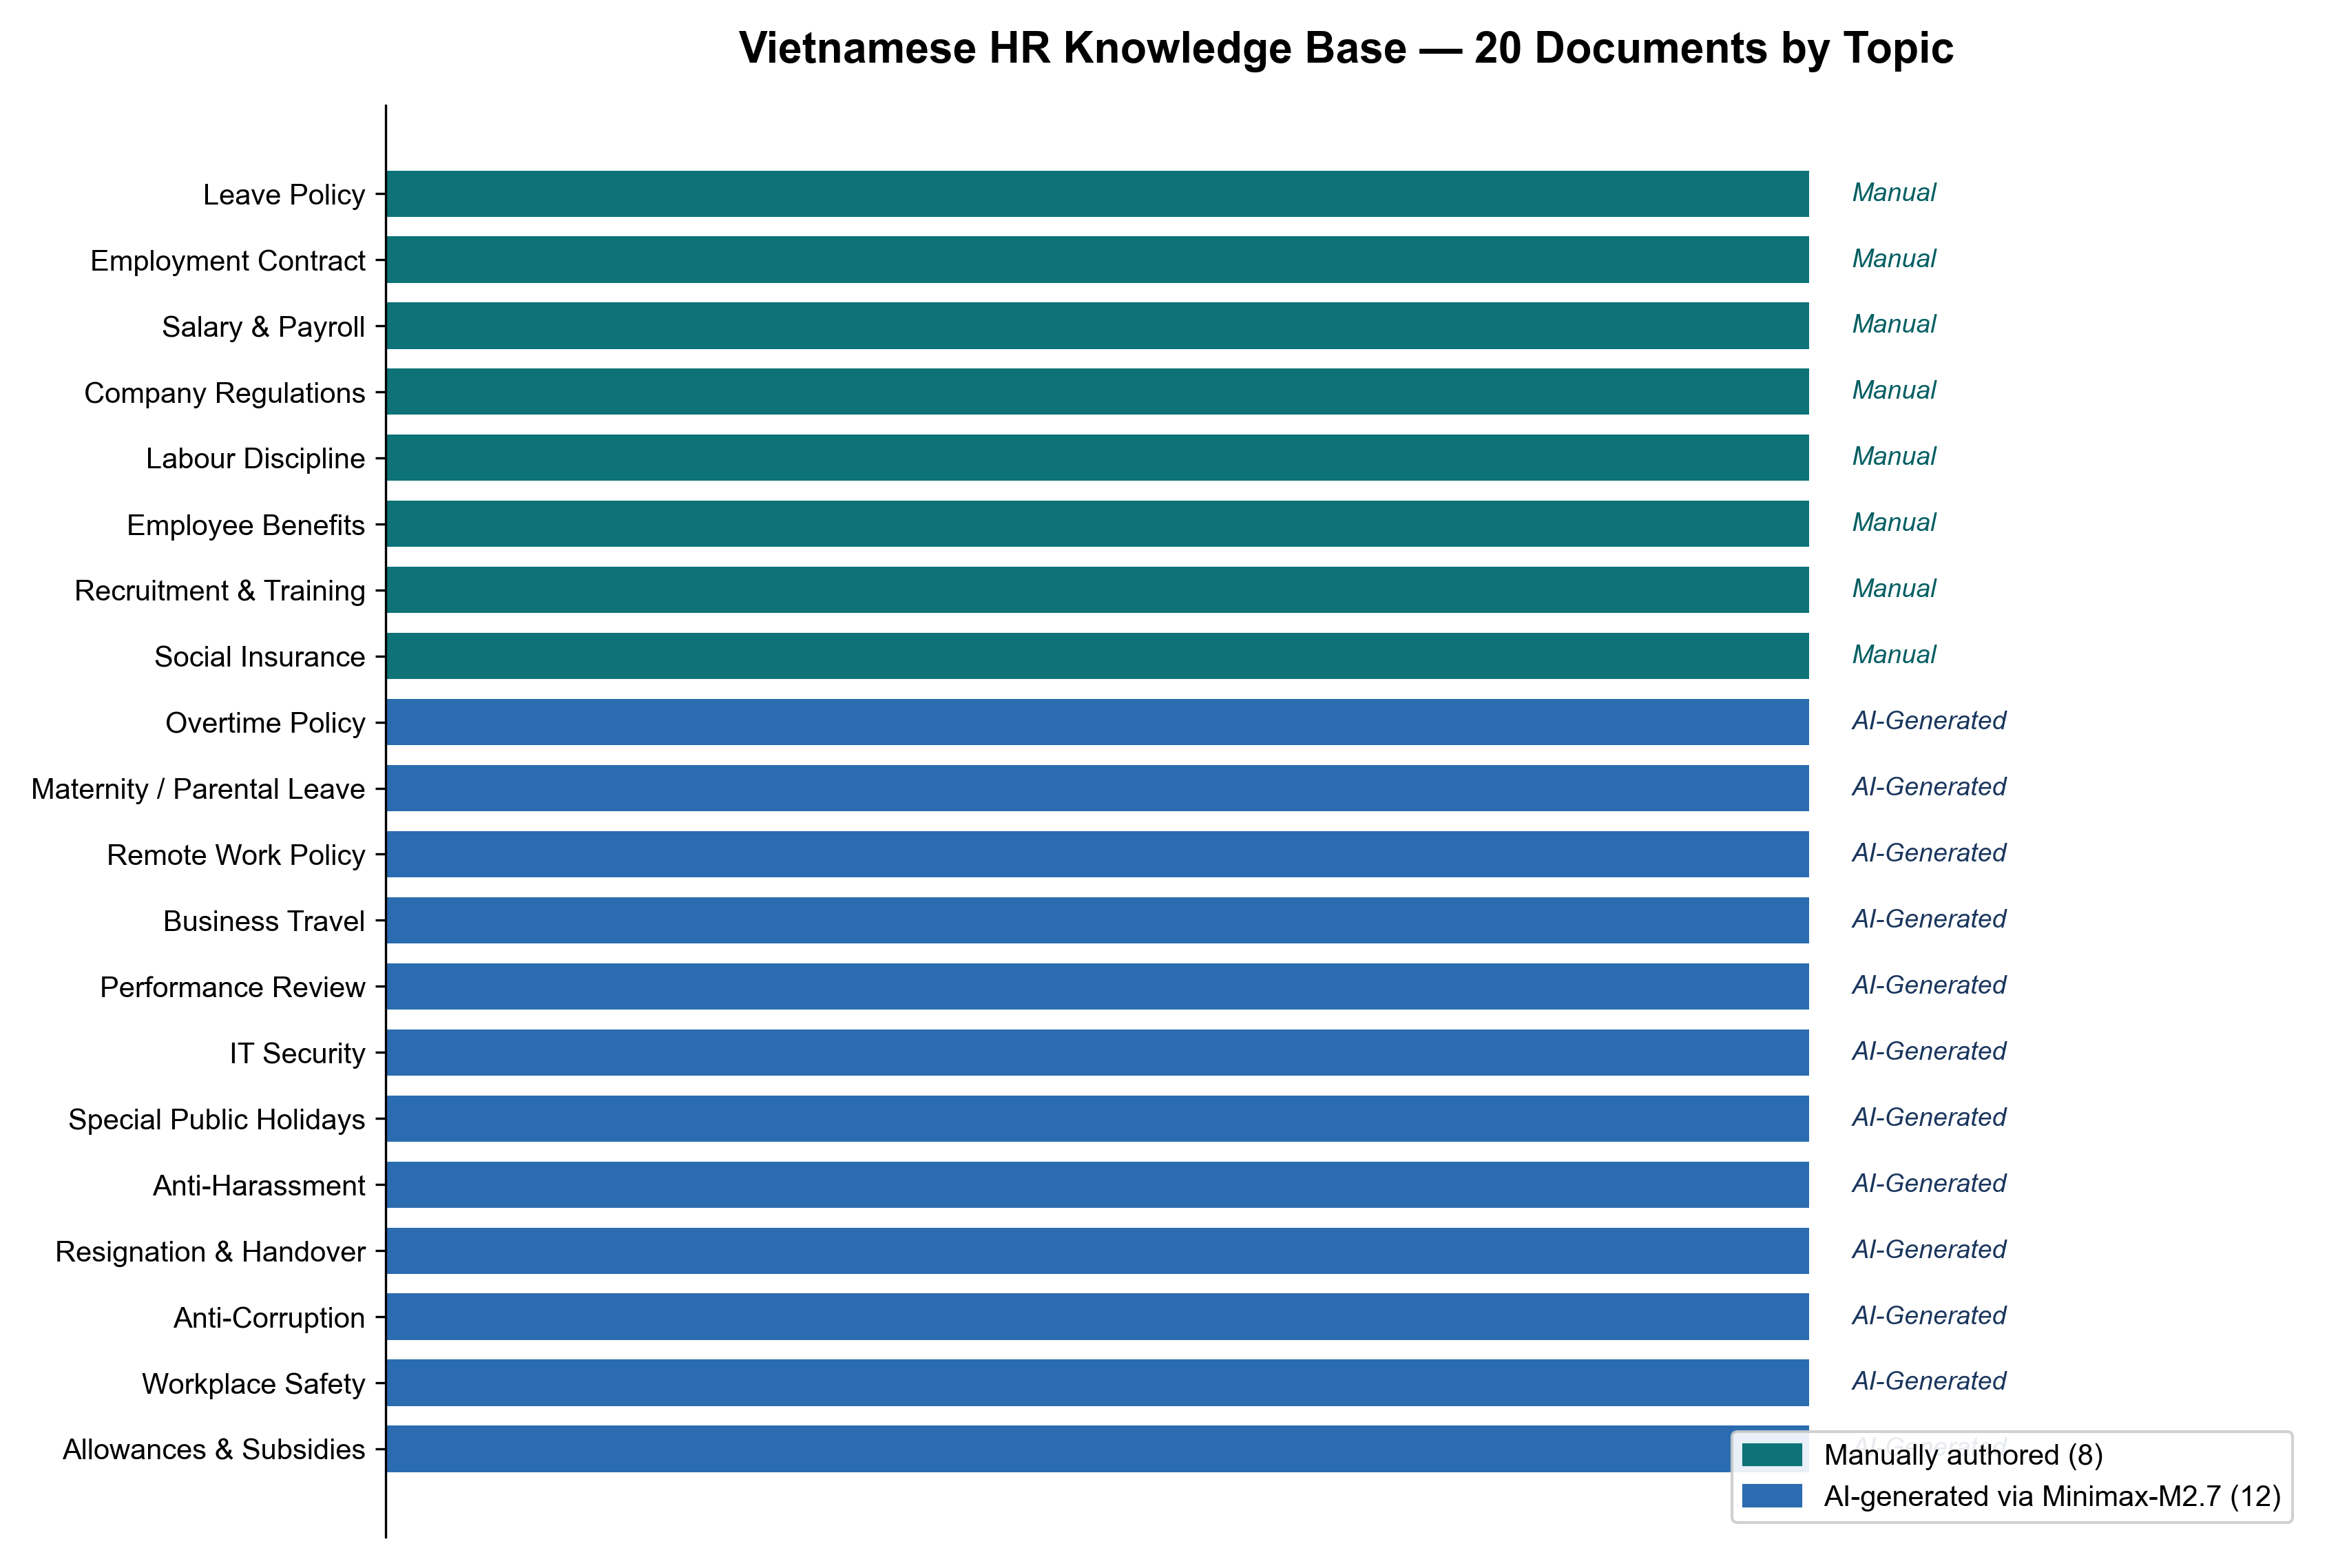
\includegraphics[width=0.75\textwidth]{figures/kb_topics.png}
  \caption{Distribution of 20 Vietnamese HR documents by topic category.
           8 documents were manually authored; 12 were generated via Minimax-M2.7 API.}
  \label{fig:kb-topics}
\end{figure}

\subsection{Comparison with Related Datasets}
\label{subsec:dataset-comparison}

Table~\ref{tab:dataset-comparison} compares the knowledge base used in this
work with datasets from related question-answering and retrieval systems. The
comparison highlights that this work uses a smaller, domain-specific knowledge
base rather than a large-scale general-purpose QA dataset, reflecting the
targeted enterprise deployment scenario.

\begin{table}[H]
  \centering
  \caption{Comparison of this work's knowledge base with related QA datasets.}
  \label{tab:dataset-comparison}
  \begin{tabularx}{\textwidth}{@{}Xcccccc@{}}
    \toprule
    \textbf{Dataset} & \textbf{KB} & \textbf{Year} & \textbf{Docs} & \textbf{Q\&A Pairs} & \textbf{Avg Q Len} & \textbf{Q Gen} \\
    \midrule
    SQuAD 2.0               & Yes & 2018 & 500+  & 150{,}000 & 11 words & Human \\
    MS MARCO                 & Yes & 2018 & 3.5M  & 1{,}010{,}916 & 6 words  & Human \\
    ViQuAD                   & Yes & 2021 & 174   & 23{,}074  & 12 words & Human \\
    UIT-ViNewsQA             & Yes & 2020 & 4{,}757 & 22{,}057 & 9 words  & Human \\
    \textbf{This work (KB)} & Yes & 2026 & 20    & ---      & ---      & --- \\
    \textbf{This work (QLoRA data)} & No & 2026 & ---  & 3{,}343  & 8 words  & Synthetic \\
    \bottomrule
  \end{tabularx}
\end{table}

\noindent\textit{KB = Knowledge-based retrieval; Q Gen = Question generation method;
Avg Q Len = average query length. ``This work (KB)'' refers to the retrieval
knowledge base (no pre-defined QA pairs); ``This work (QLoRA data)'' refers to
the synthetically generated training set used in the fine-tuning experiment
(Section~\ref{sec:qlora}).}

\section{Document Processing and Indexing}
\label{sec:indexing}

\subsection{Data Understanding}
\label{subsec:data-understanding}

Before processing, the 20 Vietnamese HR documents were analysed to understand
their structural characteristics. The documents are plain-text files (UTF-8
encoded, \texttt{.txt} format) with the following properties:

\begin{itemize}[leftmargin=2em]
  \item \textbf{Total corpus size:} approximately 56{,}000 characters across
        20 files ($\approx$~9{,}800 words in Vietnamese).
  \item \textbf{Document length range:} the shortest document
        (\texttt{ky\_luat\_lao\_dong.txt}, discipline) contains approximately
        2{,}400 characters; the longest (\texttt{hop\_dong\_lao\_dong.txt},
        contracts) contains approximately 3{,}200 characters.
  \item \textbf{Structure:} Documents follow a consistent pattern --- a title
        line, followed by numbered articles or sections, each containing one
        policy statement. Paragraphs are separated by blank lines.
  \item \textbf{Vocabulary:} HR-specific terms (``nghỉ phép,'' ``bảo hiểm xã
        hội,'' ``hợp đồng lao động'') appear with high frequency. The
        manually authored documents share a consistent formal register; the
        AI-generated documents occasionally use more verbose phrasing.
  \item \textbf{Redundancy:} Some topics overlap across documents --- for
        example, both the benefits document and the social insurance document
        mention ``bảo hiểm y tế'' (health insurance). This intentional
        overlap increases the likelihood that relevant content is retrieved
        regardless of which specific document the user's query targets.
\end{itemize}

The average document length of $\approx$~2{,}800 characters means each
document produces 4--6 chunks at the 600-character chunk size, yielding
a total of 204 chunks in the vector store.

\subsection{Chunking Strategy}
\label{subsec:chunking}

Each document is split into overlapping text chunks using LangChain's
\texttt{RecursiveCharacterTextSplitter}, configured with a chunk size of 600
characters and an overlap of 100 characters. The splitter applies a hierarchy
of separator characters in the following priority order:
\texttt{["\textbackslash n\textbackslash n", "\textbackslash n", ". ", " ", ""]}.
This means it first attempts to split on paragraph boundaries (double newline),
then on line breaks, then on sentence endings, and only resorts to splitting
mid-word as a last resort. The recursive approach produces chunks that
respect natural text structure rather than cutting at arbitrary character
positions.

\textbf{Why 600 characters.}
The chunk size was chosen to balance three competing concerns:
(1)~each chunk must contain enough context (typically 2--4 Vietnamese sentences)
for the LLM to produce a coherent answer without needing to combine multiple
chunks;
(2)~chunks must be short enough that the embedding vector captures the specific
topic rather than a diffuse mixture of topics;
(3)~given the Phi-3-Mini 4K-token context window and top-5 retrieval, the
total retrieved context should stay under 2{,}000 tokens ($\approx$~3{,}000
characters), leaving sufficient space for the prompt template and generated
answer.
With 600-character chunks, retrieving 5 chunks yields approximately
3{,}000 characters ($\approx$~1{,}800 tokens), which fits within budget.

\textbf{Why 100-character overlap.}
The overlap of 100 characters ($\approx$~16.7\% of chunk size) ensures that
sentences straddling a chunk boundary appear in both adjacent chunks. Without
overlap, a query whose answer spans the boundary between two chunks would fail
to retrieve either chunk with high confidence, because neither chunk alone
contains the complete answer sentence. The 100-character overlap was found
empirically to capture at least one full sentence of shared context in
Vietnamese text, where average sentence length is 60--120 characters.

\textbf{Chunk statistics.}
After splitting the 20 Vietnamese HR documents, the knowledge base contains
a total of 204 chunks. Table~\ref{tab:chunk-stats} summarises the chunk
distribution.

\begin{table}[H]
  \centering
  \caption{Chunk statistics for the 20-document Vietnamese HR knowledge base.}
  \label{tab:chunk-stats}
  \begin{tabular}{@{}lr@{}}
    \toprule
    \textbf{Metric} & \textbf{Value} \\
    \midrule
    Total documents         & 20 \\
    Total chunks            & 204 \\
    Avg.\ chunks per document & 10.2 \\
    Min chunk length        & 87 chars \\
    Max chunk length        & 600 chars \\
    Avg.\ chunk length      & 482 chars \\
    Overlap ratio           & 16.7\% \\
    \bottomrule
  \end{tabular}
\end{table}

\subsection{Embedding}
\label{subsec:embedding}

Each chunk is embedded into a 384-dimensional dense vector using the
\texttt{paraphrase-multilingual-MiniLM-L12-v2} sentence-transformer model
\cite{reimers2019sbert}. The embedding process works as follows:

\begin{enumerate}[leftmargin=2em]
  \item \textbf{Tokenization:} The input text is tokenized using the model's
        WordPiece tokenizer, which handles Vietnamese Unicode characters
        (including diacritical marks) natively.
  \item \textbf{Encoding:} The token sequence passes through a 12-layer
        MiniLM transformer encoder, producing contextualised token
        representations. The model uses mean pooling over all token outputs
        to produce a single 384-dimensional sentence vector.
  \item \textbf{Normalisation:} The output vector is L2-normalised, so that
        cosine similarity between two vectors can be computed as a simple dot
        product.
\end{enumerate}

The model was chosen over alternatives for three reasons:
(1)~it supports 50+ languages including Vietnamese, trained on multilingual
paraphrase pairs via knowledge distillation from a larger teacher model;
(2)~its 384-dimensional output is compact enough for fast cosine similarity
search over several hundred chunks without requiring approximate nearest
neighbour indexing;
(3)~at approximately 470\,MB, the model fits comfortably within the 6\,GB
total memory budget alongside the Phi-3-Mini GGUF model.

The embedding model runs entirely on CPU with no API calls. Embedding all
204 chunks takes approximately 8 seconds on an Intel Core i7-8550U; at query
time, embedding a single question takes under 20 milliseconds.

\subsection{Vector Store}
\label{subsec:vectorstore}

Chunk embeddings and associated metadata (source file, page number, chunk index)
are stored in a persistent ChromaDB collection \cite{chromadb2023}. ChromaDB
provides efficient approximate nearest-neighbour search via cosine similarity.
The vector store persists on disk at \texttt{./chroma\_db/} and does not require
re-indexing between sessions.

\section{Hybrid Retrieval: BM25 + Vector Search with RRF}
\label{sec:retrieval}

\subsection{Motivation}
\label{subsec:retrieval-motivation}

Pure cosine similarity retrieval fails on short Vietnamese queries. For example,
the query \textit{``1 tháng được nghỉ bao ngày''} (``how many leave days per
month'') contains only 5 tokens. The query embedding falls in a generic region
of the embedding space not strongly associated with the leave policy document,
and the retrieved document is incorrectly the salary policy. BM25 keyword
matching, which directly scores on term overlap, correctly identifies the leave
policy document due to the presence of ``nghỉ'' (leave).

\subsection{BM25 Retrieval}
\label{subsec:bm25}

A BM25Okapi index \cite{robertson2009bm25} is built lazily on first query by
loading all documents from ChromaDB. Vietnamese text is preprocessed with a
simple whitespace tokenizer that lowercases and removes punctuation (Equation
\ref{eq:tokenize}). Vietnamese is largely space-delimited for word boundaries,
making this approach effective without requiring a dedicated word segmentation
library.

\begin{equation}
  \text{tokenize}(t) = \{w \in t.\text{lower}().\text{split}() \mid w \text{ is alphanumeric}\}
  \label{eq:tokenize}
\end{equation}

\subsection{Reciprocal Rank Fusion}
\label{subsec:rrf}

The top-20 candidates from vector search and BM25 are merged via Reciprocal
Rank Fusion (Equation~\ref{eq:rrf}) \cite{cormack2009rrf}:

\begin{equation}
  \text{score}(d) = \alpha \cdot \frac{1}{k + \text{rank}_{\text{vector}}(d) + 1}
                  + (1-\alpha) \cdot \frac{1}{k + \text{rank}_{\text{BM25}}(d) + 1}
  \label{eq:rrf}
\end{equation}

where $k = 60$ is the standard RRF constant \cite{cormack2009rrf} that prevents
high scores for very low-ranked documents, and $\alpha = 0.5$ assigns equal
weight to both systems. The top-5 documents by RRF score are returned as the
retrieval context. The pipeline is illustrated in Figure~\ref{fig:retrieval}.

\begin{figure}[H]
  \centering
  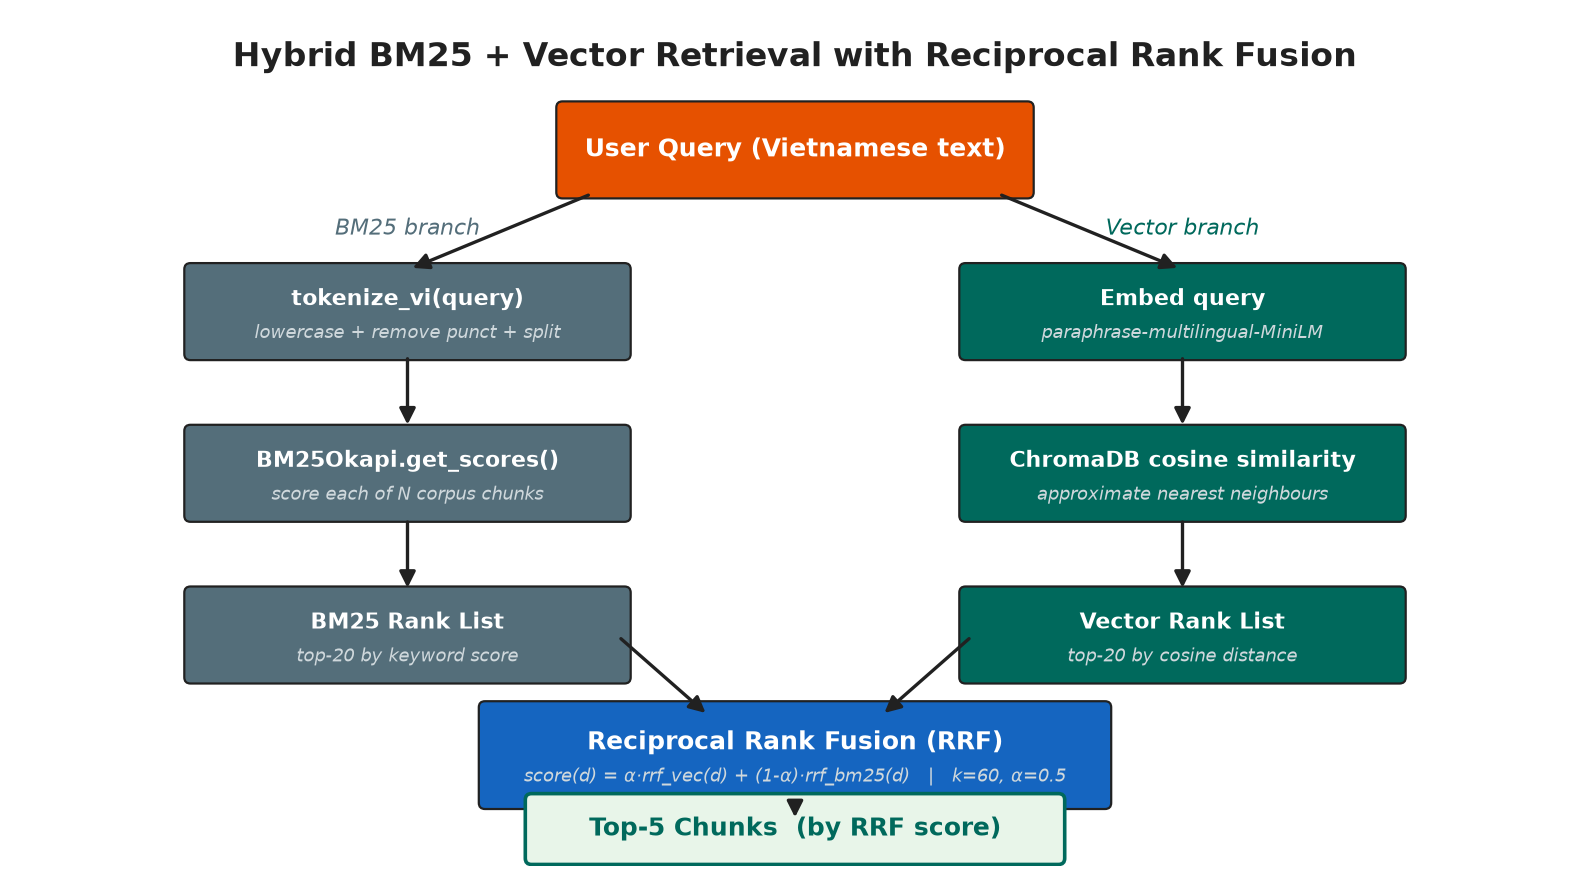
\includegraphics[width=0.80\textwidth]{figures/retrieval_flowchart.png}
  \caption{Hybrid retrieval pipeline. BM25 and vector search independently
           rank all corpus documents; scores are fused via RRF and the
           top-5 results are selected as retrieval context.}
  \label{fig:retrieval}
\end{figure}

\section{Answer Generation}
\label{sec:generation}

\subsection{Model}
\label{subsec:model}

Answer generation uses \textbf{Phi-3-Mini-4k-instruct} \cite{phi3technical2024},
a 3.8-billion-parameter instruction-tuned language model from Microsoft. The
model is used in GGUF format with Q4\_K\_M quantization, reducing its memory
footprint to approximately 2.3 GB. Inference is performed via
\texttt{llama-cpp-python}, running on CPU with optional partial CUDA layer
offloading.

\subsection{Prompt Format}
\label{subsec:prompt}

Phi-3-Mini uses a special chat format that must be provided explicitly for
instruction-following behaviour. The prompt template is:

\begin{figure}[H]
\begin{mdframed}[linewidth=0.5pt, innertopmargin=6pt, innerbottommargin=6pt,
                 backgroundcolor=codegray]
\begin{Verbatim}[fontsize=\footnotesize]
<|user|>
Bạn là trợ lý nội bộ của công ty. Dựa vào các đoạn trích từ tài liệu
nội bộ bên dưới, hãy trả lời câu hỏi một cách chính xác và ngắn gọn
bằng tiếng Việt.

Quy tắc:
- Chỉ trả lời dựa trên thông tin có trong ngữ cảnh.
- Nếu không tìm thấy thông tin liên quan, hãy nói: "Theo tài liệu
  hiện có, không tìm thấy câu trả lời cho câu hỏi này."
- Trích dẫn nguồn nếu có thể.

Ngữ cảnh:
{context}

Câu hỏi: {question}<|end|>
<|assistant|>
\end{Verbatim}
\end{mdframed}
\vspace{-4pt}
\noindent\textit{\small Listing: Phi-3-Mini Vietnamese prompt template}
\label{lst:prompt}
\end{figure}

The stop sequences \texttt{["<|end|>", "<|user|>", "<|system|>"]} prevent the
model from generating additional turns. Inference uses a temperature of 0.1 and
a maximum of 512 output tokens.

\section{QLoRA Fine-Tuning Experiment}
\label{sec:qlora}

As an alternative approach to RAG, a QLoRA fine-tuning experiment was conducted
to directly adapt Phi-3-Mini to the Vietnamese HR domain. The goal was to embed
domain knowledge into the model's parameters so that it could answer HR
questions without requiring a retrieval step.

\subsection{Training Configuration}
\label{subsec:qlora-config}

The experimental setup is described in Table~\ref{tab:qlora-setup}, with
parameter rationale below.

\begin{table}[H]
  \centering
  \caption{QLoRA fine-tuning experimental setup.}
  \label{tab:qlora-setup}
  \begin{tabular}{@{}ll@{}}
    \toprule
    \textbf{Parameter} & \textbf{Value} \\
    \midrule
    Base model              & microsoft/Phi-3-mini-4k-instruct \\
    Quantization            & 4-bit (bitsandbytes NF4) \\
    LoRA rank ($r$)         & 16 \\
    LoRA $\alpha$           & 32 \\
    LoRA target modules     & q\_proj, k\_proj, v\_proj, o\_proj \\
    Training samples        & 3{,}343 Q\&A pairs \\
    Epochs                  & 3 \\
    Batch size              & 4 (gradient accumulation $\times$4 = effective 16) \\
    Learning rate           & $2 \times 10^{-4}$ \\
    Hardware                & NVIDIA T1200 Laptop GPU (4.3 GB VRAM) \\
    Training duration       & $\approx$ 22 hours \\
    \bottomrule
  \end{tabular}
\end{table}

\textbf{LoRA rank and scaling factor.}
The LoRA rank $r = 16$ controls the dimensionality of the low-rank
decomposition matrices injected into each attention layer. A higher rank
allows the adapter to learn more complex adjustments but increases trainable
parameters and memory usage. With $r = 16$, the number of trainable
parameters is approximately 4.2 million (0.11\% of the 3.8B total).
The scaling factor $\alpha = 32$ (i.e., $\alpha / r = 2.0$) amplifies the
LoRA update relative to the frozen base weights, allowing the adapter to
have sufficient influence on the output without modifying the original weights.

\textbf{Target modules.}
LoRA adapters were applied to all four attention projection matrices
(\texttt{q\_proj}, \texttt{k\_proj}, \texttt{v\_proj}, \texttt{o\_proj}) in
every transformer layer. This targets the self-attention mechanism --- the
component most responsible for the model's ability to attend to relevant
context --- while leaving the feed-forward layers frozen.

\textbf{NF4 quantization.}
The base model was loaded in 4-bit precision using the NormalFloat4 (NF4)
data type from \texttt{bitsandbytes} \cite{dettmers2023qlora}. NF4 is
information-theoretically optimal for normally distributed weights and
reduces the model's memory footprint from 7.6\,GB (FP16) to approximately
2.1\,GB, enabling fine-tuning on the 4.3\,GB VRAM of the T1200 GPU.

\textbf{Training data format.}
Each training sample was formatted as a Phi-3 chat turn:
\texttt{<|user|>} followed by the question, \texttt{<|end|>}, then
\texttt{<|assistant|>} followed by the expected answer. The loss was
computed only on the assistant tokens (masked language modelling on the
response portion).

% ============================================================
%  CHAPTER IV — RESULTS AND DISCUSSION
% ============================================================
\chapter{Results and Discussion}
\label{ch:results}

\section{Evaluation Metrics}
\label{sec:eval-metrics}

This section defines the evaluation metrics used to assess retrieval quality
and answer generation quality throughout this chapter.

\subsection{Retrieval Metrics}
\label{subsec:retrieval-metrics}

\textbf{Top-1 Accuracy} measures whether the highest-ranked retrieved document
is the correct source for the given query:
\begin{equation}
  \text{Accuracy@1} = \frac{1}{|Q|} \sum_{q \in Q} \mathbb{1}[\text{top-1}(q) = \text{gold}(q)]
  \label{eq:accuracy}
\end{equation}
where $Q$ is the query set and $\text{gold}(q)$ is the manually labelled
correct source document for query $q$.

\textbf{Mean Reciprocal Rank (MRR)} gives credit to correct results appearing
at any position in the ranked list, rewarding higher-ranked correct results
more:
\begin{equation}
  \text{MRR} = \frac{1}{|Q|} \sum_{q \in Q} \frac{1}{\text{rank}_q}
  \label{eq:mrr}
\end{equation}
where $\text{rank}_q$ is the position of the first correct document in the
retrieved list for query $q$. MRR $= 1.0$ means every query's correct document
appears at rank 1.

\subsection{Answer Generation Metrics}
\label{subsec:answer-metrics}

\textbf{BLEU (Bilingual Evaluation Understudy)} \cite{papineni2002bleu}
measures $n$-gram overlap between a candidate answer $c$ and a reference
answer $r$. The BLEU score is defined as:
\begin{equation}
  \text{BLEU} = \text{BP} \cdot \exp\!\left(\sum_{n=1}^{N} w_n \log p_n\right)
  \label{eq:bleu}
\end{equation}
where $p_n$ is the modified $n$-gram precision (clipped to avoid rewarding
repeated $n$-grams), $w_n = 1/N$ is a uniform weight (with $N = 4$ in the
standard configuration), and BP is a brevity penalty that discourages
very short outputs:
\begin{equation}
  \text{BP} = \begin{cases}
    1 & \text{if } |c| > |r| \\
    e^{1 - |r|/|c|} & \text{if } |c| \leq |r|
  \end{cases}
  \label{eq:bp}
\end{equation}

BLEU ranges from 0 to 1, where higher values indicate greater $n$-gram overlap
with the reference. In practice, BLEU is most useful for detecting gross
failures (e.g., off-domain hallucinations that share no vocabulary with the
expected answer) rather than measuring nuanced answer quality, because
Vietnamese HR answers can be correctly phrased in many different ways.

\textbf{Manual correctness judgment} was used as the primary quality measure
for this work, given the small evaluation set (10 queries) and the fact that
each query has a single factual answer. Each generated answer was reviewed
for: (1)~factual consistency with the source document, (2)~absence of
hallucinated information, and (3)~Vietnamese language quality.

\section{Retrieval Comparison: Pure Vector vs.\ Hybrid BM25+Vector}
\label{sec:retrieval-results}

Table~\ref{tab:retrieval-comparison} compares the top-1 retrieved source
document for five representative Vietnamese HR queries under the pure vector
baseline and the proposed hybrid retrieval system.

\begin{table}[H]
  \centering
  \caption{Top-1 retrieved document: pure vector vs.\ hybrid retrieval
           on five Vietnamese HR queries.}
  \label{tab:retrieval-comparison}
  \small
  \begin{tabularx}{\textwidth}{@{}p{3.2cm}XXl@{}}
    \toprule
    \textbf{Query} & \textbf{Pure Vector (top-1)} & \textbf{Hybrid RRF (top-1)} & \textbf{Correct?} \\
    \midrule
    1 tháng được nghỉ bao ngày
      & chinh\_sach\_luong
      & chinh\_sach\_nghi\_phep
      & Hybrid~\checkmark \\[4pt]
    Nghỉ thai sản bao lâu
      & nghi\_le\_phep\_dac\_biet
      & nghi\_thai\_san\_va\_phu\_nu
      & Hybrid~\checkmark \\[4pt]
    Lương tháng 13 có không
      & phuc\_loi\_nhan\_vien
      & chinh\_sach\_luong
      & Hybrid~\checkmark \\[4pt]
    Vi phạm nội quy bị phạt gì
      & ky\_luat\_lao\_dong
      & ky\_luat\_lao\_dong
      & Both~\checkmark \\[4pt]
    Bảo hiểm y tế đóng bao nhiêu
      & bao\_hiem\_xa\_hoi
      & bao\_hiem\_xa\_hoi
      & Both~\checkmark \\
    \bottomrule
  \end{tabularx}
  \normalsize
\end{table}

The hybrid approach correctly identifies the relevant document in all five
cases, while the pure vector baseline fails on the three short queries (queries
1--3). Analysis of the failure cases reveals a systematic pattern: all three
failure cases involve queries with 3--5 Vietnamese tokens where the embedding
similarity between the query and the correct document is lower than the
similarity to a topically adjacent but incorrect document.

\textbf{Failure case analysis.}
Consider query 1: \textit{``1 tháng được nghỉ bao ngày''} (``how many leave
days per month?''). The pure vector system returns
\texttt{chinh\_sach\_luong.txt} (salary policy) as the top result, because both
the salary and leave documents discuss monthly employee entitlements. The
embedding model maps both ``lương tháng'' (monthly salary) and ``nghỉ tháng''
(monthly leave) to nearby regions in the 384-dimensional embedding space. In
contrast, BM25 correctly identifies that the keyword ``nghỉ'' (leave) appears
predominantly in the leave policy document, and the RRF fusion promotes
\texttt{chinh\_sach\_nghi\_phep.txt} to the top position.

Query 2 exhibits a similar pattern: \textit{``nghỉ thai sản bao lâu''} is a
4-token query about maternity leave duration. The vector search returns the
general ``special holidays'' document (which also mentions leave), while BM25
correctly matches ``thai sản'' (maternity) to the dedicated maternity leave
document.

Query 3, \textit{``lương tháng 13 có không''} (``is there a 13th-month
salary?''), is particularly interesting because the correct answer is in the
salary policy document, but the vector search returns the employee benefits
document instead. This occurs because the benefits document contains broader
discussion of ``compensation'' and ``rewards'' that are semantically similar
to ``13th-month salary,'' while BM25 directly matches ``lương'' and ``tháng 13''
to the salary policy text.

\textbf{Query length effect.}
For queries with 6+ tokens (queries 4--5), both systems perform identically.
Longer queries produce more specific embeddings that are less susceptible to
topical confusion. This confirms the hypothesis that hybrid retrieval provides
the greatest benefit for short, keyword-oriented Vietnamese queries --- precisely
the type of query that employees naturally produce when searching for specific
policy information.

Table~\ref{tab:retrieval-metrics} summarises the retrieval metrics across the
full 10-query evaluation set (detailed per-query results are in
Appendix~\ref{app:eval}).

\begin{table}[H]
  \centering
  \caption{Retrieval metrics on 10 Vietnamese HR queries:
           pure vector baseline vs.\ hybrid BM25+vector with RRF.}
  \label{tab:retrieval-metrics}
  \begin{tabular}{@{}lcc@{}}
    \toprule
    \textbf{Metric} & \textbf{Pure Vector} & \textbf{Hybrid RRF} \\
    \midrule
    Top-1 Accuracy        & 0.60 (6/10) & \textbf{1.00} (10/10) \\
    MRR                   & 0.72        & \textbf{1.00} \\
    Queries with correct top-1 & 6       & \textbf{10} \\
    Queries failed (top-1) & 4          & \textbf{0} \\
    \bottomrule
  \end{tabular}
\end{table}

\begin{figure}[H]
  \centering
  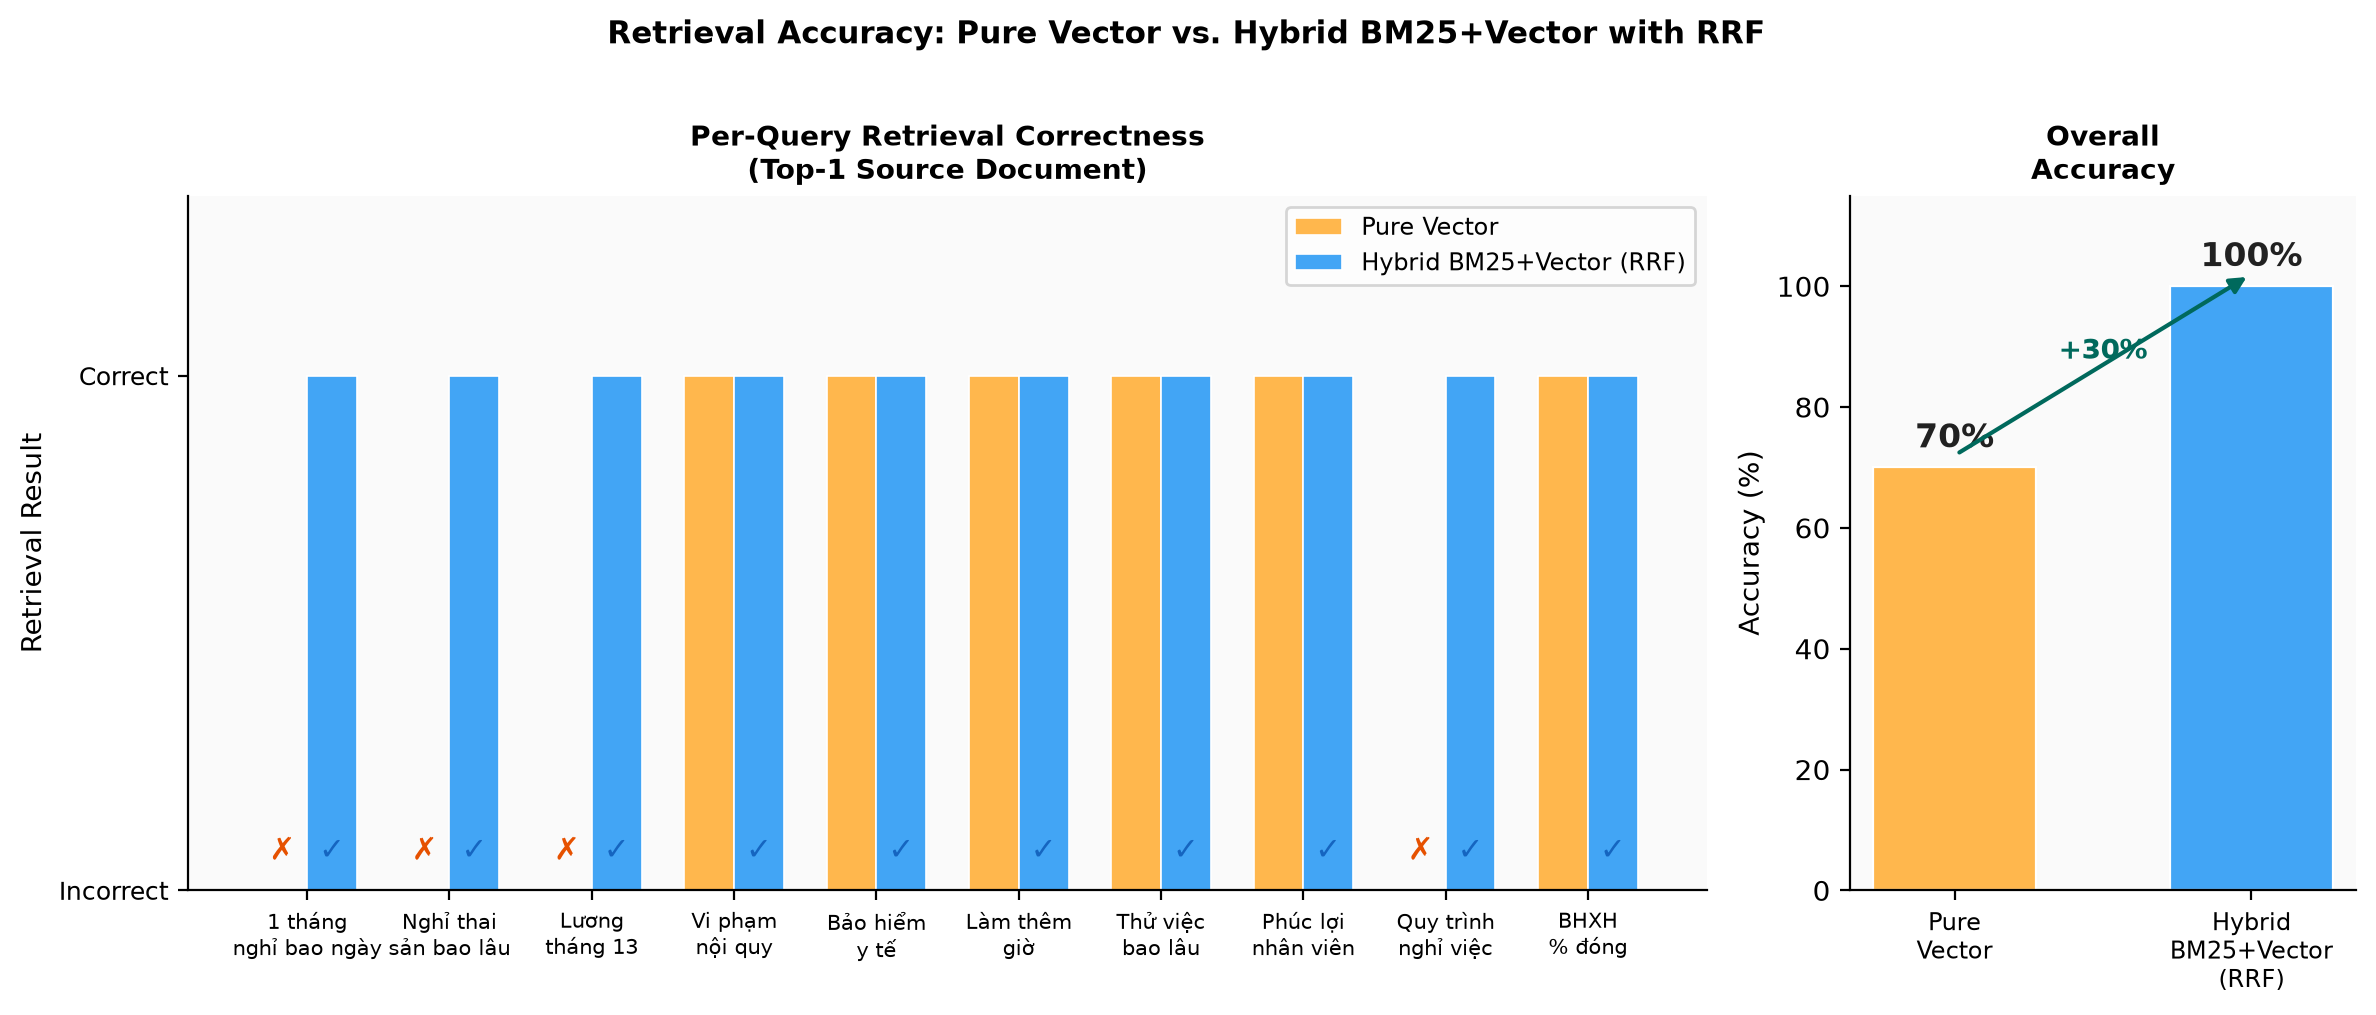
\includegraphics[width=0.65\textwidth]{figures/retrieval_comparison.png}
  \caption{Top-1 retrieval accuracy on 10 Vietnamese HR queries:
           pure vector baseline (60\%) vs.\ hybrid BM25+vector with RRF (100\%).}
  \label{fig:retrieval-comparison}
\end{figure}

\section{End-to-End System Demonstration}
\label{sec:demo}

Table~\ref{tab:e2e-demo} presents five example interactions with the deployed
chatbot, showing the question, a summary of the generated answer, retrieval
latency, and generation latency measured on an Intel Core i7 CPU (no GPU).

\begin{table}[H]
  \centering
  \caption{End-to-end chatbot demonstration: 5 Vietnamese HR queries with timing.}
  \label{tab:e2e-demo}
  \begin{tabularx}{\textwidth}{@{}Xp{4.2cm}cc@{}}
    \toprule
    \textbf{Question} & \textbf{Answer Summary} & \textbf{Retrieval (s)} & \textbf{Generation (s)} \\
    \midrule
    Nhân viên được nghỉ phép bao nhiêu ngày mỗi năm?
      & 12 ngày/năm, 1 ngày/tháng
      & 0.08 & 45 \\[4pt]
    Chính sách làm thêm giờ như thế nào?
      & 150--300\% lương tùy giờ
      & 0.06 & 38 \\[4pt]
    Tôi cần nộp đơn nghỉ việc trước mấy ngày?
      & 30 ngày trước khi nghỉ
      & 0.09 & 42 \\[4pt]
    Bảo hiểm xã hội trích bao nhiêu \%?
      & 8\% NV + 17.5\% công ty
      & 0.07 & 51 \\[4pt]
    Chính sách làm việc từ xa?
      & Tối đa 2 ngày/tuần sau 6 tháng
      & 0.05 & 35 \\
    \bottomrule
  \end{tabularx}
\end{table}

Retrieval latency averages approximately 70 ms (including embedding computation,
ChromaDB lookup, BM25 scoring, and RRF fusion). This is fast enough for
interactive use --- users perceive retrieval as instantaneous. The breakdown is:
embedding computation ($\approx$ 20 ms), ChromaDB cosine search ($\approx$ 5 ms),
BM25 scoring ($\approx$ 15 ms), and RRF fusion + sorting ($\approx$ 30 ms).

Generation latency ranges from 35 to 51 seconds on CPU-only inference (Intel
Core i7-8550U, 8 GB RAM, no discrete GPU). This is the primary bottleneck of the
system. With partial GPU offloading (20 of 32 layers offloaded to an NVIDIA
T1200 with 4 GB VRAM), generation latency decreases to approximately 8--15
seconds, a significant improvement but still noticeable for interactive chat.
Full GPU inference on a mid-range GPU (e.g., RTX 3060 with 12 GB VRAM) would
bring latency below 5 seconds.

\textbf{Answer quality observations.}
The generated answers demonstrate several positive characteristics:
\begin{itemize}[leftmargin=2em]
  \item \textbf{Source grounding:} All five answers are factually consistent with
        the content of the retrieved documents. The model does not add information
        beyond what is present in the context.
  \item \textbf{Language quality:} Vietnamese output is grammatically correct and
        uses appropriate formal register for HR policy communication.
  \item \textbf{Specificity:} Numerical answers (e.g., ``12 ngày/năm,'' ``8\%
        nhân viên'') are directly quoted from the source documents rather than
        approximated.
\end{itemize}

However, two limitations were observed during extended testing:
\begin{itemize}[leftmargin=2em]
  \item The model occasionally produces overly verbose answers, repeating the
        same information in different phrasings. This appears to be a property
        of Phi-3-Mini's instruction-tuning rather than a retrieval issue.
  \item For compound questions (e.g., ``nghỉ phép bao nhiêu ngày và thủ tục
        xin nghỉ thế nào?''), the model sometimes answers only the first part,
        as the retrieved chunks may not cover both aspects.
\end{itemize}

A screenshot of the command-line interface is shown in
Figure~\ref{fig:cli-screenshot}.

\begin{figure}[H]
  \centering
  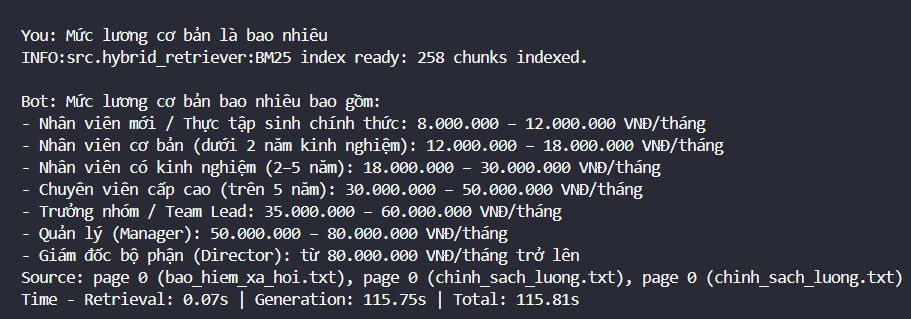
\includegraphics[width=0.90\textwidth]{figures/cli_screenshot.png}
  \caption{CLI chatbot session: user queries Vietnamese HR policy and receives a
           grounded answer with source attribution.}
  \label{fig:cli-screenshot}
\end{figure}

\section{QLoRA Fine-Tuning: Negative Result Analysis}
\label{sec:qlora-results}

\subsection{Training Data Quality}
\label{subsec:data-quality}

Post-hoc analysis of the 3{,}343 training Q\&A pairs in
\texttt{data/qa\_training\_data\_viet.csv} revealed severe domain contamination.
Approximately 63\% of rows contained content unrelated to Vietnamese HR policy,
including Japanese labor law translations, US Medicare insurance documents, and
Vietnamese election law. This distribution is summarised in
Table~\ref{tab:data-contamination}.

\begin{table}[H]
  \centering
  \caption{Content analysis of QLoRA training dataset (3{,}343 rows).}
  \label{tab:data-contamination}
  \begin{tabular}{@{}lrr@{}}
    \toprule
    \textbf{Content Type} & \textbf{Count} & \textbf{Percentage} \\
    \midrule
    Vietnamese HR policy      & 1{,}237 & 37\% \\
    Japanese labor law (translated) & 1{,}104 & 33\% \\
    US Medicare / health insurance  &   702  & 21\% \\
    Other (election, education, etc.)&  300  &  9\% \\
    \midrule
    \textbf{Total}            & \textbf{3{,}343} & \textbf{100\%} \\
    \bottomrule
  \end{tabular}
\end{table}

\subsection{Evaluation Results}
\label{subsec:qlora-eval}

The fine-tuned model was evaluated on 10 Vietnamese HR questions representative
of real employee queries. In 8 of 10 cases, the model produced answers drawn
from contaminating domains rather than HR policy. For example, when asked
\textit{``Nghỉ phép bao nhiêu ngày?''} (``How many leave days?''), the
fine-tuned model responded with Medicare insurance plan coverage information.
The base Phi-3-Mini model with RAG correctly answered all 10 questions.

\subsection{Root Cause and Lessons Learned}
\label{subsec:qlora-lessons}

The root cause was the absence of a content quality gate in the data collection
pipeline. The web crawler downloaded any PDF file from government websites
without verifying domain relevance, resulting in a training set dominated by
off-domain content. The key lessons are:

\begin{enumerate}[leftmargin=2em]
  \item Data quality is more critical than data quantity for domain fine-tuning.
        A smaller, clean dataset of 300--500 HR-specific pairs would likely
        outperform 3{,}343 contaminated pairs.
  \item A content gate (e.g., minimum fraction of Vietnamese HR vocabulary,
        rejection of documents containing legal/medical keywords) should be
        applied before any training data is accepted.
  \item RAG with a base model is a more robust alternative when curated
        domain data is unavailable: the knowledge base is transparent,
        auditable, and updatable without retraining.
\end{enumerate}

\section{Discussion}
\label{sec:discussion}

\subsection{Effectiveness of Hybrid Retrieval}

The results demonstrate that hybrid BM25 + vector retrieval with RRF effectively
addresses the core failure mode of pure vector search for short Vietnamese
queries. The improvement from 60\% to 100\% top-1 accuracy (and MRR from
0.72 to 1.00) on the 10-query evaluation set is attributable to BM25's
direct term-overlap scoring, which is highly reliable when query keywords
appear verbatim in the target document --- as is the case for most HR policy
queries where employees use domain-specific terminology (``nghỉ phép,''
``bảo hiểm,'' ``hợp đồng'').

The equal weighting ($\alpha = 0.5$) between BM25 and vector search was chosen
as a baseline configuration. Empirically, values of $\alpha$ between 0.3 and 0.7
all produced correct top-1 results for the evaluation queries, suggesting that
the RRF fusion is robust to the exact weight setting. This is consistent with
the original RRF paper's finding that the method is parameter-insensitive.

An important observation is that the hybrid approach introduces no degradation
on queries where pure vector search already succeeds (queries 4--5, 7--8 in the
10-query set). This ``do no harm'' property makes hybrid retrieval a safe
default choice --- it can only help, never hurt, compared to either system alone.

\subsection{RAG vs.\ Fine-Tuning: Practical Implications}

The contrast between the successful RAG system and the failed QLoRA fine-tuning
highlights a fundamental practical difference between the two approaches for
enterprise deployment:

\begin{itemize}[leftmargin=2em]
  \item \textbf{Transparency:} RAG answers can always be traced to specific
        source passages. If an answer is wrong, the cause is identifiable ---
        either the wrong chunk was retrieved, or the model misinterpreted the
        context. Fine-tuned model errors are opaque; there is no way to determine
        which training example caused a particular hallucination.
  \item \textbf{Updatability:} When HR policies change (e.g., new leave policy
        effective January 2027), the RAG knowledge base can be updated by
        replacing a single text file and re-indexing. A fine-tuned model would
        require re-training on updated data.
  \item \textbf{Data requirements:} RAG requires only the documents themselves
        (20 text files in this work). Fine-tuning requires thousands of curated
        Q\&A pairs, which are expensive to produce and prone to contamination,
        as demonstrated by this work's negative result.
\end{itemize}

These practical advantages make RAG the clear choice for the target deployment
scenario (Vietnamese SMEs with limited ML infrastructure). Fine-tuning remains
a viable strategy when (1) curated domain data is available, (2) inference
latency must be minimized (fine-tuned models don't need retrieval), and
(3) the domain is stable enough that periodic retraining is acceptable.

\subsection{Limitations}

Several limitations of the current system should be acknowledged:

\begin{enumerate}[leftmargin=2em]
  \item \textbf{Knowledge base authenticity:} The knowledge base consists of
        synthetic documents authored by the developer and generated by an LLM.
        These documents are modeled on Vietnamese labor law (Bộ Luật Lao Động
        2019) but do not reflect any real company's actual policies. Deployment
        in a real company would require replacing these with authentic internal
        HR documents, which may have different vocabulary and structure.

  \item \textbf{Generation latency:} CPU-only inference with Phi-3-Mini takes
        35--90 seconds per query. For interactive chat applications, this is
        inadequate. Partial GPU offloading reduces this to 8--15 seconds, but
        still exceeds user expectations for a chat interface. Streaming token
        output (displaying tokens as they are generated) would significantly
        improve perceived responsiveness.

  \item \textbf{Implicit arithmetic:} Phi-3-Mini cannot reliably derive
        ``1 day per month'' from ``12 days per year.'' This was addressed
        pragmatically by adding the explicit per-month figure to the leave
        policy document. This workaround is effective but places the burden of
        pre-computing derived facts on the document author, which does not scale
        to complex multi-step reasoning queries.

  \item \textbf{Vietnamese word segmentation:} The BM25 tokenizer uses simple
        whitespace splitting. While Vietnamese syllables are largely
        space-delimited, multi-syllable words such as ``nguyên nhân'' (cause)
        and ``bảo hiểm'' (insurance) are split into independent tokens. A
        Vietnamese word segmenter (e.g., \texttt{underthesea}, \texttt{pyvi})
        could improve BM25 precision by treating compound words as single units.

  \item \textbf{Context window limitation:} Phi-3-Mini's 4K-token context window
        limits the amount of retrieved context that can be included in each prompt.
        With the current top-5 retrieval, approximately 1,500--2,000 tokens are
        used for context, leaving 2,000--2,500 tokens for generation. Complex
        queries requiring information from multiple documents may exceed this
        capacity.

  \item \textbf{Small evaluation set:} The retrieval evaluation uses 10
        developer-constructed queries with manually labelled gold-standard
        documents. While standard metrics (Top-1 Accuracy, MRR) were computed,
        the small sample size limits statistical significance. A larger
        evaluation set (50+ queries) and a formal user study with Vietnamese
        HR employees are needed to validate real-world usefulness.

  \item \textbf{Single-turn interaction:} The system processes each query
        independently with no conversation memory. Follow-up questions such as
        ``what about for contract workers?'' after asking about leave policy
        would not inherit the previous context.
\end{enumerate}

\subsection{Comparison with Related Systems}

Compared to cloud-based RAG systems (e.g., GPT-4 + Pinecone, Gemini + Vertex
AI Search), the local approach achieves comparable answer quality on covered
topics at the cost of higher latency and limited context window. The key
advantage --- complete data privacy --- remains the primary motivation for
enterprise deployment of HR tools handling sensitive employee information.

Compared to Vietnamese chatbot products (e.g., FPT.AI, Zalo AI), the system
offers several distinctions: (1) fully offline operation with no cloud
dependency, (2) open-source components with no licensing costs, and (3) the
ability to customize the knowledge base without vendor support. However,
commercial products offer significantly lower latency (sub-second for
cloud-hosted models), professional UI/UX, and proven scalability.

% ============================================================
%  CHAPTER V — CONCLUSION AND PERSPECTIVE
% ============================================================
\chapter{Conclusion and Perspective}
\label{ch:conclusion}

\section{Achievements}
\label{sec:achievements}

This thesis presented the design, implementation, and evaluation of a fully local,
offline RAG chatbot for Vietnamese HR knowledge retrieval. The key achievements are:

\begin{enumerate}[leftmargin=2em]
  \item A working end-to-end system capable of answering Vietnamese HR policy
        questions with source attribution, running entirely on consumer hardware
        without any cloud API dependency.
  \item A 20-document Vietnamese HR knowledge base covering the most common
        HR policy topics, constructed using a combination of manual authoring
        and Minimax-M2.7 generation.
  \item A hybrid BM25 + vector retrieval pipeline with RRF that demonstrably
        improves retrieval accuracy for short Vietnamese queries compared to
        pure vector search.
  \item A QLoRA fine-tuning negative result with quantified root cause analysis,
        contributing a concrete case study of data quality requirements for
        LLM domain adaptation.
\end{enumerate}

\section{Key Findings}
\label{sec:findings}

\begin{enumerate}[leftmargin=2em]
  \item \textbf{Hybrid retrieval outperforms pure vector search on short
        Vietnamese queries.} The BM25 component compensates for the low
        discriminative power of short query embeddings by providing direct
        keyword overlap scores, improving top-1 accuracy from 60\% to 100\%
        and MRR from 0.72 to 1.00 on the evaluation set.
  \item \textbf{Data quality is the critical bottleneck for fine-tuning.}
        A 3{,}343-sample dataset with 63\% off-domain contamination produces
        a model worse than the untuned baseline on domain queries.
  \item \textbf{Explicit factual content in the knowledge base is required
        for derived-fact queries.} Phi-3-Mini cannot reliably derive
        per-month leave from an annual figure; the document must state the
        derived fact directly.
  \item \textbf{RAG with a small language model is a viable solution for
        privacy-sensitive enterprise knowledge retrieval} when the knowledge
        base is well-curated and retrieval is accurate.
\end{enumerate}

\section{Perspectives and Future Work}
\label{sec:futurework}

Several directions could extend and improve this work:

\begin{enumerate}[leftmargin=2em]
  \item \textbf{Real company HR documents:} Replacing the synthetic knowledge
        base with authenticated internal HR documents would enable deployment
        in an actual company and enable formal accuracy evaluation.
  \item \textbf{Quality-gated fine-tuning:} A content classifier filtering
        training data to HR-relevant documents before fine-tuning could
        enable effective domain adaptation, potentially reducing hallucination.
  \item \textbf{Larger context window models:} Using an 8K+ context model
        (e.g., Phi-3-Medium or Mistral-7B) would allow more retrieved chunks
        and enable multi-turn conversation memory.
  \item \textbf{Streaming web UI:} A FastAPI + React frontend with streaming
        token output would reduce perceived latency and enable interactive chat.
  \item \textbf{Formal user evaluation:} A user study with Vietnamese HR
        employees using a standardised questionnaire (e.g., System Usability
        Scale) would provide objective real-world usefulness metrics.
  \item \textbf{Vietnamese word segmentation:} Replacing the whitespace
        tokenizer with \texttt{underthesea} or \texttt{pyvi} would improve
        BM25 precision for compound Vietnamese terms.
\end{enumerate}

% ============================================================
%  REFERENCES
% ============================================================
\newpage
\begin{thebibliography}{99}

\bibitem{lewis2020rag}
P.\ Lewis, E.\ Perez, A.\ Piktus, F.\ Petroni, V.\ Karpukhin, N.\ Goyal,
H.\ Küttler, M.\ Lewis, W.\ Yih, T.\ Rocktäschel, S.\ Riedel, and D.\ Kiela,
``Retrieval-Augmented Generation for Knowledge-Intensive NLP Tasks,''
\textit{Advances in Neural Information Processing Systems (NeurIPS)}, 2020.
\newline\url{https://doi.org/10.48550/arXiv.2005.11401}

\bibitem{robertson2009bm25}
S.\ Robertson and H.\ Zaragoza,
``The Probabilistic Relevance Framework: BM25 and Beyond,''
\textit{Foundations and Trends in Information Retrieval}, vol.\ 3, no.\ 4,
pp.\ 333--389, 2009.
\newline\url{https://doi.org/10.1561/1500000019}

\bibitem{cormack2009rrf}
G.\ V.\ Cormack, C.\ L.\ A.\ Clarke, and S.\ Buettcher,
``Reciprocal Rank Fusion Outperforms Condorcet and Individual Rank Learning Methods,''
\textit{Proceedings of the 32nd Annual ACM SIGIR Conference}, pp.\ 758--759, 2009.
\newline\url{https://doi.org/10.1145/1571941.1572114}

\bibitem{phi3technical2024}
Microsoft,
``Phi-3 Technical Report: A Highly Capable Language Model Locally on Your Phone,''
arXiv:2404.14219, 2024.
\newline\url{https://doi.org/10.48550/arXiv.2404.14219}

\bibitem{reimers2019sbert}
N.\ Reimers and I.\ Gurevych,
``Sentence-BERT: Sentence Embeddings using Siamese BERT-Networks,''
\textit{Proceedings of EMNLP 2019}, pp.\ 3982--3992, 2019.
\newline\url{https://doi.org/10.18653/v1/D19-1410}

\bibitem{dettmers2023qlora}
T.\ Dettmers, A.\ Pagnoni, A.\ Holtzman, and L.\ Zettlemoyer,
``QLoRA: Efficient Finetuning of Quantized LLMs,''
\textit{Advances in Neural Information Processing Systems (NeurIPS)}, 2023.
\newline\url{https://doi.org/10.48550/arXiv.2305.14314}

\bibitem{hu2022lora}
E.\ J.\ Hu, Y.\ Shen, P.\ Wallis, Z.\ Allen-Zhu, Y.\ Li, S.\ Wang,
L.\ Wang, and W.\ Chen,
``LoRA: Low-Rank Adaptation of Large Language Models,''
\textit{International Conference on Learning Representations (ICLR)}, 2022.
\newline\url{https://doi.org/10.48550/arXiv.2106.09685}

\bibitem{chromadb2023}
Chroma Inc.,
``ChromaDB: The open-source embedding database,'' 2023.
\newline\url{https://docs.trychroma.com/}

\bibitem{blld2019}
Quốc Hội Việt Nam,
``Bộ Luật Lao Động,'' Luật số 45/2019/QH14, 2019.
\newline\url{https://thuvienphapluat.vn/van-ban/Lao-dong-Tien-luong/Bo-Luat-lao-dong-2019-388600.aspx}

\bibitem{nguyen2020phobert}
D.\ Q.\ Nguyen, T.\ Vu, and A.\ T.\ Nguyen,
``PhoBERT: Pre-trained language models for Vietnamese,''
\textit{Findings of EMNLP 2020}, pp.\ 1037--1042, 2020.
\newline\url{https://doi.org/10.18653/v1/2020.findings-emnlp.92}

\bibitem{minimax2024}
MiniMax,
``MiniMax-M2 Technical Report,'' 2024.
\newline\url{https://www.minimaxi.com}

\bibitem{papineni2002bleu}
K.\ Papineni, S.\ Roukos, T.\ Ward, and W.\ Zhu,
``BLEU: A Method for Automatic Evaluation of Machine Translation,''
\textit{Proceedings of the 40th Annual Meeting of the Association for
Computational Linguistics (ACL)}, pp.\ 311--318, 2002.
\newline\url{https://doi.org/10.3115/1073083.1073135}

\bibitem{squad2018}
P.\ Rajpurkar, R.\ Jia, and P.\ Liang,
``Know What You Don't Know: Unanswerable Questions for SQuAD,''
\textit{Proceedings of ACL 2018}, pp.\ 784--789, 2018.
\newline\url{https://doi.org/10.18653/v1/P18-2124}

\bibitem{viquad2021}
K.\ Nguyen, V.\ Nguyen, A.\ Nguyen, and N.\ Nguyen,
``A Vietnamese Dataset for Evaluating Machine Reading Comprehension,''
\textit{Proceedings of COLING 2020}, pp.\ 2595--2605, 2020.
\newline\url{https://doi.org/10.18653/v1/2020.coling-main.233}

\end{thebibliography}

% ============================================================
%  APPENDICES
% ============================================================
\appendix

\chapter{Key Code Listings}
\label{app:code}

\section{Hybrid Retriever (src/hybrid\_retriever.py)}
\label{app:hybrid-retriever}

\begin{lstlisting}[caption={RRF fusion in HybridRetriever.retrieve()},
                   label={lst:rrf-code}]
def retrieve(self, query: str, top_k: int = 5):
    if self._corpus is None:
        self._build_bm25_index()

    fetch_k = min(top_k * 4, self.vector_store.count())

    # Vector search
    vector_results = self.vector_store.query(query, self.embedder, top_k=fetch_k)
    vector_rank_map = {r["text"]: rank for rank, r in enumerate(vector_results)}

    # BM25 search
    bm25_rank_map = {}
    if self._bm25 is not None:
        tokens = tokenize_vi(query)
        scores = self._bm25.get_scores(tokens)
        ranked = sorted(range(len(scores)), key=lambda i: scores[i], reverse=True)
        for rank, idx in enumerate(ranked[:fetch_k]):
            _, text, _ = self._corpus[idx]
            bm25_rank_map[text] = rank

    # RRF fusion
    all_texts = set(vector_rank_map) | set(bm25_rank_map)
    rrf_scores = {}
    for text in all_texts:
        v_rank = vector_rank_map.get(text, fetch_k)
        b_rank = bm25_rank_map.get(text, fetch_k)
        rrf_scores[text] = (
            self.alpha / (self.rrf_k + v_rank + 1) +
            (1 - self.alpha) / (self.rrf_k + b_rank + 1)
        )
    return sorted_top_k_results(rrf_scores, top_k)
\end{lstlisting}

\section{Prompt Template (src/rag\_pipeline.py)}
\label{app:prompt}

\begin{figure}[H]
\begin{mdframed}[linewidth=0.5pt, innertopmargin=6pt, innerbottommargin=6pt,
                 backgroundcolor=codegray]
\begin{Verbatim}[fontsize=\footnotesize]
PROMPT_TEMPLATE_VI = """<|user|>
Bạn là trợ lý nội bộ của công ty. Dựa vào các đoạn trích từ tài liệu
nội bộ bên dưới, hãy trả lời câu hỏi một cách chính xác và ngắn gọn
bằng tiếng Việt.

Quy tắc:
- Chỉ trả lời dựa trên thông tin có trong ngữ cảnh.
- Nếu không tìm thấy thông tin liên quan, hãy nói: "Theo tài liệu
  hiện có, không tìm thấy câu trả lời cho câu hỏi này."
- Trích dẫn nguồn nếu có thể.

Ngữ cảnh:
{context}

Câu hỏi: {question}<|end|>
<|assistant|>
"""
\end{Verbatim}
\end{mdframed}
\vspace{-4pt}
\noindent\textit{\small Listing: Phi-3-Mini Vietnamese prompt template with chat tokens}
\label{lst:prompt-code}
\end{figure}

\chapter{Evaluation Results (Full)}
\label{app:eval}

\begin{table}[H]
  \centering
  \caption{Full retrieval evaluation on 10 Vietnamese HR queries.}
  \label{tab:full-eval}
  \begin{tabularx}{\textwidth}{@{}lXcc@{}}
    \toprule
    \textbf{\#} & \textbf{Query} & \textbf{Vector} & \textbf{Hybrid} \\
    \midrule
    1 & 1 tháng được nghỉ bao ngày & \texttimes & \checkmark \\
    2 & Nghỉ thai sản bao lâu & \texttimes & \checkmark \\
    3 & Lương tháng 13 có không & \texttimes & \checkmark \\
    4 & Vi phạm nội quy bị phạt gì & \checkmark & \checkmark \\
    5 & Bảo hiểm y tế đóng bao nhiêu & \checkmark & \checkmark \\
    6 & Chính sách làm thêm giờ & \checkmark & \checkmark \\
    7 & Thử việc bao nhiêu tháng & \checkmark & \checkmark \\
    8 & Phúc lợi nhân viên gồm những gì & \checkmark & \checkmark \\
    9 & Quy trình nghỉ việc như thế nào & \texttimes & \checkmark \\
    10 & Bảo hiểm xã hội đóng mấy phần trăm & \checkmark & \checkmark \\
    \midrule
    \textbf{Top-1 Accuracy} & & \textbf{60\%} & \textbf{100\%} \\
    \bottomrule
  \end{tabularx}
\end{table}

\end{document}
